% Separate supporting document; compile from the manuscript directory.
\documentclass[10pt]{article}
\usepackage[a4paper,margin=23mm]{geometry}
\usepackage[T1]{fontenc}
\usepackage[utf8]{inputenc}
\usepackage{lmodern}
\usepackage{amsmath,amssymb,graphicx,booktabs}
\usepackage[numbers,sort&compress]{natbib}
\usepackage[font=small,labelfont=bf]{caption}
\usepackage[colorlinks=true,linkcolor=blue,citecolor=blue,urlcolor=blue]{hyperref}
\newcommand{\rscan}{\ensuremath{r^{2}}SCAN}
\renewcommand{\thesection}{S\arabic{section}}
\renewcommand{\thesubsection}{\thesection.\arabic{subsection}}
\renewcommand{\thefigure}{S\arabic{figure}}
\renewcommand{\thetable}{S\arabic{table}}
\renewcommand{\theequation}{S\arabic{equation}}
\setlength{\parskip}{4pt}
\setlength{\parindent}{1em}
\renewcommand{\topfraction}{0.9}
\renewcommand{\bottomfraction}{0.85}
\renewcommand{\textfraction}{0.08}
\renewcommand{\floatpagefraction}{0.7}
\begin{document}
\begin{center}
{\Large\bfseries Supporting Materials}\par\medskip
{\large Assessing exchange-correlation effects in Ti--Al alloys with fine-tuned foundation interatomic potentials}\par\medskip
N. N. Katkov$^{1}$, E. O. Khazieva$^{1}$, and R. E. Ryltsev$^{1,2}$\par
{\small $^{1}$Vatolin Institute of Metallurgy of the Ural Branch of the Russian Academy of Sciences, Amundsena Street 101, Yekaterinburg 620016, Russia\par
$^{2}$Ural Federal University, 620002 Ekaterinburg, Russia\par
Corresponding author: \href{mailto:rrylcev@mail.ru}{rrylcev@mail.ru}}\par\medskip
Draft -- 1 November 2026
\end{center}

This document supports selection of PBE 15k through learning curves, complete training/validation errors, and the hcp-Ti PBE DFT phonon DOS. The selection balances these diagnostics: 15k improves energy and force accuracy over 5k and gives the smallest integral DOS discrepancies among the five saved checkpoints, while later checkpoints give smaller energy errors. The current benchmark uses PBE 20k on 30 completed common structures; the physical-property selection and the earlier fixed 20-structure audit remain separate. The supporting data also include the 60~ps r2SCAN enthalpy series and three PBE 15k alloy-viscosity estimates with 15 replicas each. The new matched DFT/DPA4 phonon comparison for all three functionals is documented in Sec.~\ref{sec:matched_phonons}; the earlier checkpoint-selection diagnostics below retain their original protocols. Table~\ref{tab:coverage} identifies the remaining 5k results.

\section{Checkpoint identity, learning curves, and selection}
\label{sec:selection}
The PBE fine-tuning schedule ran to approximately 23\,400 optimization steps. We denote the saved checkpoints by 5k, 10k, 15k, 20k, and 23.4k; their stored zero-based step indices are 4999, 9999, 14\,999, 19\,999, and 23\,399. The 5k checkpoint is identical, by SHA-256, to the originally supplied PBE model. The selected checkpoint for the updated physical properties is 15k; the DFT-reference benchmark uses 20k. The allocation, including retained 5k properties, is listed in Table~\ref{tab:coverage}. The final PBEsol and \rscan{} checkpoints have stored indices 23\,099 and 23\,199, respectively, and were retained after their learning curves reached a plateau. The fine-tuning protocol was common to the three functionals, as detailed in the main Methods.

The training--validation comparison motivated an audit of all five saved PBE checkpoints. Selection of 15k combines improved absolute training and validation errors relative to 5k with the best integral agreement with the \emph{PBE DFT DOS of hcp Ti}, evaluated both at identical DFT geometry and at each model's equilibrium cell. Experimental dispersion points are a secondary comparison, not the selection criterion.

At 15k, complete-set energy RMSEs are 3.322/3.512~meV/atom for training/validation, compared with 5.214/6.071 at 5k. Force-component RMSEs are 0.05989/0.06487~eV/\AA, compared with 0.06298/0.06669 at 5k. Further training to 23.4k changes the validation force RMSE only to 0.06468~eV/\AA, but reduces the validation energy RMSE to 1.233~meV/atom. Thus, ``optimal'' refers to the adopted balance between error and phonon criteria, not to a unique minimum of validation loss or the train--validation gap. The increasing force-error gap does not establish general overfitting. The checkpoint audit included held-out errors and is retrospective; no parameters or offsets were fitted to the holdout, but these comparisons are not a new, untouched post-selection test.

Figure~\ref{fig:learning} shows that a growing force-error gap is compatible with decreasing validation error. Over steps 3000--5000, mean logged training/validation energy MAEs are approximately 2.96/3.67~meV/atom and force MAEs are 0.0946/0.0985~eV/\AA. Near the end of training (steps 20\,001--23\,400), energy MAEs fall to 0.827/0.980~meV/atom and force MAEs to 0.0865/0.0945~eV/\AA. The force gap widens as training error decreases more rapidly. These logged metrics are descriptive training diagnostics; with the force-norm loss option enabled, they are not interchangeable with pooled Cartesian-component errors from complete-dataset inference. Section~\ref{sec:errors} provides the latter comparison and does not support a general worsening of energy/force prediction after 5k.

\begin{figure}[htbp]
\centering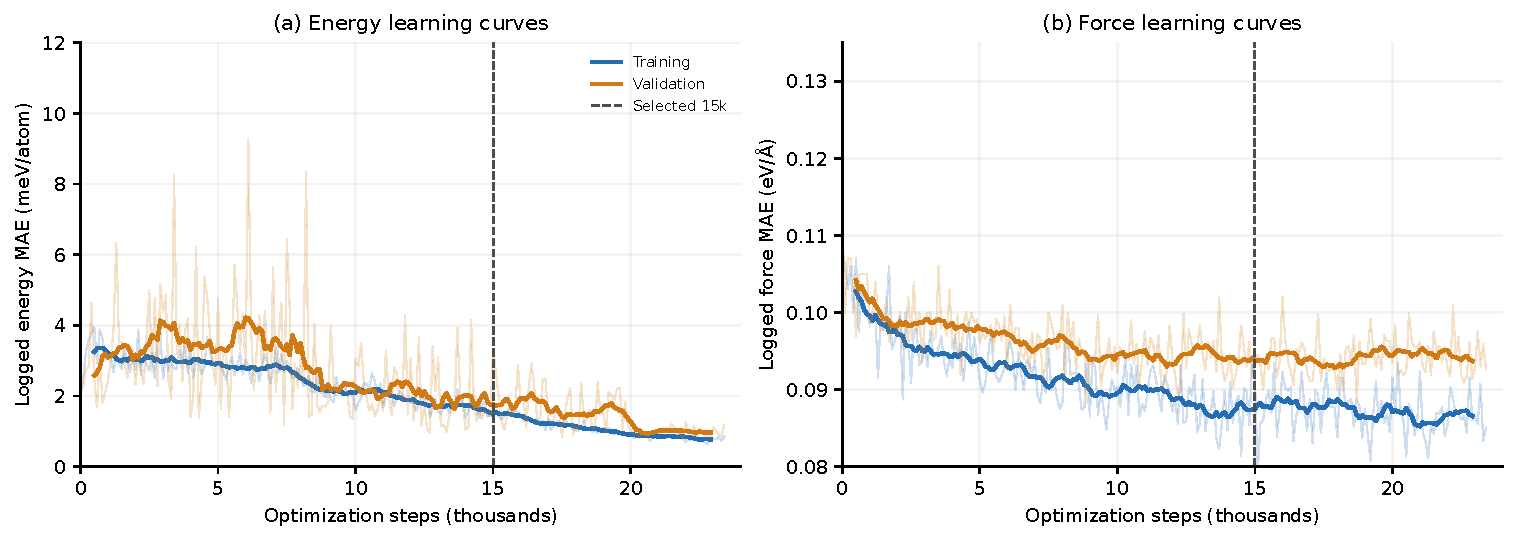
\includegraphics[width=\linewidth]{figures/supporting/learning_curves.pdf}
\caption{PBE learning curves from the complete training log. Pale lines show recorded values; solid lines show centered 11-record moving means, without extrapolation at the ends. The vertical line marks the selected 15k checkpoint. The axes emphasize the later training regime; the initial transient may extend beyond the plotted ranges. The force ordinate is the metric printed in the training log, not the Cartesian-component RMSE reported below.}
\label{fig:learning}
\end{figure}

\section{Matched evaluation of the five PBE checkpoints}
\label{sec:errors}
The original checkpoint audit, retained here as a fixed diagnostic comparison, evaluated each checkpoint without relaxation on the same 850 training configurations, 149 original validation configurations, and 20 common held-out liquid-pool configurations, giving 5095 model--configuration evaluations. The test structures contain 216 atoms each. Native CPU inference used the original checkpoints with verified file identities; no retraining, energy-offset fitting, or configuration-dependent corrections were performed. The original 5k checkpoint was also checked against its frozen export, with energy differences below 0.005~meV/atom and maximum force-component differences below $10^{-4}$~eV/\AA.

The energy residual for configuration $i$ is $(E_i^{\rm model}-E_i^{\rm DFT})/N_i$, using the archived VASP free energy (\texttt{TOTEN}) and identical atomic geometry. Energy RMSEs weight configurations equally. Force RMSEs pool all Cartesian components. Stress errors use the same component convention for every checkpoint. These definitions are held fixed across Tables~\ref{tab:errors} and \ref{tab:stress}; the training-log quantities in Sec.~\ref{sec:selection} are not substituted for these metrics.

\begin{table}[htbp]
\centering
\caption{Energy and force RMSEs from complete-dataset inference. Energy: meV/atom; forces: eV/\AA. This table uses the earlier fixed 20-structure liquid test subset. The selected model is now 15k; current 23-structure errors are reported separately below and in the main article.}
\label{tab:errors}
\begin{tabular}{r rrr rrr}
\toprule
Steps ($10^3$) & \multicolumn{3}{c}{Energy RMSE} & \multicolumn{3}{c}{Force-component RMSE}\\
\cmidrule(lr){2-4}\cmidrule(lr){5-7}
 & Train & Validation & Test & Train & Validation & Test\\
\midrule
5 & 5.214 & 6.071 & 6.406 & 0.06298 & 0.06669 & 0.06754 \\
10 & 3.322 & 3.344 & 3.395 & 0.06102 & 0.06543 & 0.06627 \\
15 & 3.322 & 3.512 & 3.379 & 0.05989 & 0.06487 & 0.06552 \\
20 & 1.202 & 1.221 & 1.228 & 0.05956 & 0.06472 & 0.06538 \\
23.4 & 1.201 & 1.233 & 1.341 & 0.05949 & 0.06468 & 0.06540 \\
\bottomrule
\end{tabular}
\end{table}

\begin{table}[htbp]
\centering
\caption{Stress-component RMSEs (GPa) on the same configurations.}
\label{tab:stress}
\begin{tabular}{r rrr}
\toprule
Steps ($10^3$) & Train & Validation & Test\\
\midrule
5 & 0.08146 & 0.07632 & 0.11220 \\
10 & 0.07560 & 0.07387 & 0.08861 \\
15 & 0.06486 & 0.06023 & 0.09615 \\
20 & 0.06195 & 0.05662 & 0.08880 \\
23.4 & 0.06364 & 0.05752 & 0.08922 \\
\bottomrule
\end{tabular}
\end{table}

The final checkpoint reduces energy and force errors on all three partitions relative to 5k (Fig.~\ref{fig:sweep}). Its absolute energy residual is smaller for 649/850 training, 122/149 validation, and 18/20 test configurations. Its per-configuration force RMSE is smaller for 850/850, 147/149, and 20/20 configurations, respectively. The test energy RMSE decreases from 6.406 to 1.341~meV/atom, and the force RMSE from 0.06754 to 0.06540~eV/\AA. For comparison, the unchanged pretrained model has energy RMSEs of 2.786~meV/atom on training and 3.398~meV/atom on the test subset. The final model therefore reverses the unfavorable 5k-versus-pretrained comparison for PBE energy accuracy.

Training energy bias is not monotonic: its mean is $+2.690$, $-3.004$, $+2.821$, $+0.514$, and $+0.634$~meV/atom at the five checkpoints. This behavior cautions against interpreting one checkpoint as a limiting error of the architecture or functional. The 20k model gives a slightly smaller test energy RMSE than 23.4k, while their force errors are nearly identical. This retrospective observation does not establish 20k as an optimal replacement.

A paired bootstrap with 2000 resamples of whole test configurations gives descriptive 95\% intervals of $[-7.08,-2.67]$~meV/atom for the final-minus-5k energy-RMSE difference and $[-0.00269,-0.00161]$~eV/\AA{} for the force-RMSE difference. For final minus 20k, the intervals are $[0.0054,0.2160]$~meV/atom and $[-0.0000378,0.0000872]$~eV/\AA. These intervals are conditional on those 20 structures; they do not account for unknown trajectory correlations or retrospective checkpoint comparisons. This archived checkpoint sweep used only the 20 liquid structures completed at that time, and these statistics do not constrain solid--liquid free-energy errors.

\begin{figure}[htbp]
\centering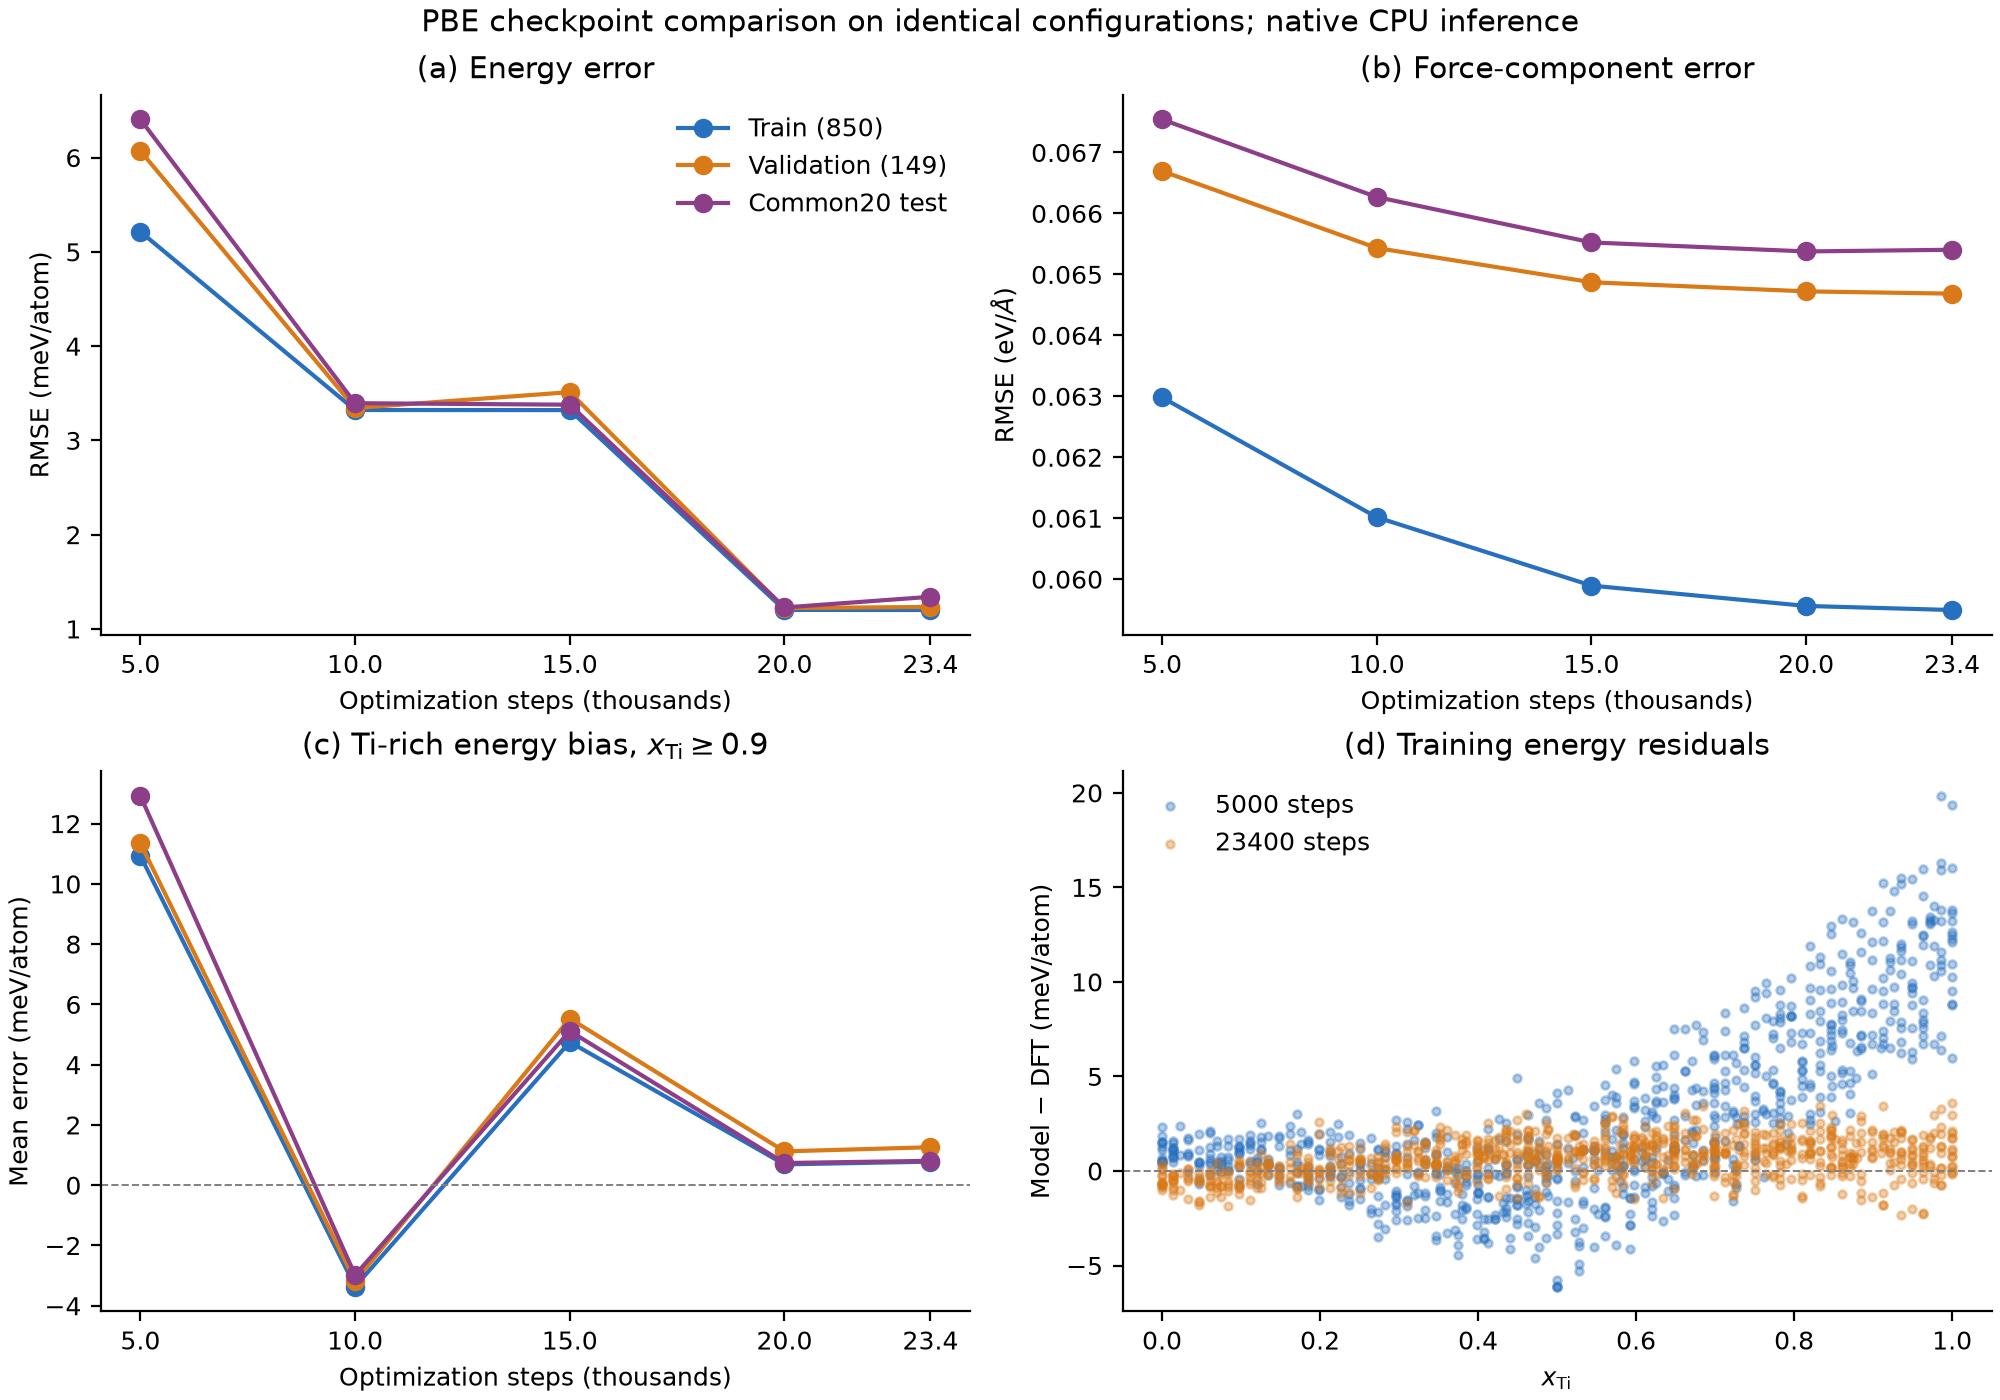
\includegraphics[width=.96\linewidth]{figures/supporting/checkpoint_comparison.png}
\caption{Matched checkpoint evaluation: (a) energy RMSE, (b) force-component RMSE, (c) mean energy residual for $x_{\rm Ti}\geq0.9$, and (d) training energy residuals versus composition at 5k and 23.4k. The Ti-rich subset in (c) contains 91 training, 24 validation, and only two test configurations; the latter is not a representative composition-resolved error estimate. Lines connect saved checkpoints and do not describe every optimization step.}
\label{fig:sweep}
\end{figure}

\section{Composition, volume, and the largest test residual}
\label{sec:bias}
The large positive energy residual of the earlier 5k model is systematic within the training data. This section retains the original 5k diagnostic and does not assign its residuals to 15k. All 91 training configurations with $x_{\rm Ti}\geq0.9$ have positive 5k residuals: their mean is $+10.93$~meV/atom and RMSE is 11.36~meV/atom, compared with a pretrained mean of $-1.20$ and RMSE of 3.32~meV/atom. On the 15 pure-Ti training configurations, the 5k RMSE is 12.39~meV/atom, compared with 5.35~meV/atom for the pretrained model. These diagnostics show that the test discrepancy is already present in fitted configurations, rather than arising solely from an isolated out-of-distribution structure.

Within the 470 training structures with $x_{\rm Ti}\geq0.5$, the 5k mean residual rises from 2.90 to 5.72 and 9.08~meV/atom in atomic-volume bins below 18, between 18 and 20, and at least 20~\AA$^3$ (220, 178, and 72 structures). Because composition and volume vary together, these bin averages alone do not isolate a volume effect. Figure~\ref{fig:volume} therefore also compares residuals at fixed composition, for Al$_{11}$Ti$_{205}$ and pure Ti. These are comparisons of sampled structures, not controlled isotropic-strain scans of a single configuration.

TiAl-test-009 has the largest 5k residual on the archived 20-structure test subset. Its composition is $x_{\rm Al}=11/216=0.0509$ and its volume is 22.1848~\AA$^3$/atom. Its DFT energy and geometry were checked, and native-checkpoint and exported-model predictions agree. There is no established data error warranting exclusion. At 5k the residual is $+17.926$~meV/atom. The 12 training configurations at the same composition already have a mean residual of $+10.012$~meV/atom; the nearest in volume, at 21.3496~\AA$^3$/atom, has a residual of $+15.454$~meV/atom. The test volume is approximately 3.9\% larger than the maximum training volume at this composition, but extrapolation alone does not explain the bias.

As a sensitivity check alone, we also evaluated errors without this structure. The 5k test RMSE then changes from 6.406 to 5.126~meV/atom, and the pretrained RMSE from 3.398 to 3.483~meV/atom. The ranking persists. All 20 structures remain included in the expanded 30-structure main benchmark. The diagnostic structure is preserved separately in POSCAR format in the accompanying analysis files.

Continued training largely removes the bias. The mean residual on the 91 Ti-rich training structures falls to $+0.781$~meV/atom at 23.4k; on the 24 Ti-rich validation structures it falls from $+11.347$ to $+1.260$~meV/atom. The test-009 residual becomes $+3.417$~meV/atom at 20k and $+3.656$~meV/atom at 23.4k. Figure~\ref{fig:volume} shows the corresponding reduction at fixed composition. This is a change in the fitted energy surface, not a post-processing shift.

As a separate diagnostic, subtracting a mean residual for each exactly repeated training composition reduces the 5k energy RMSE to 1.956~meV/atom, compared with 1.476~meV/atom for the pretrained model, on 836 structures belonging to repeated-composition groups. This diagnostic uses fitted group offsets and is \emph{not} a reported predictive error. It indicates a substantial between-composition contribution without eliminating within-composition discrepancies. No composition-dependent or elemental energy shifts are applied to any main or supporting benchmark table.

\begin{figure}[htbp]
\centering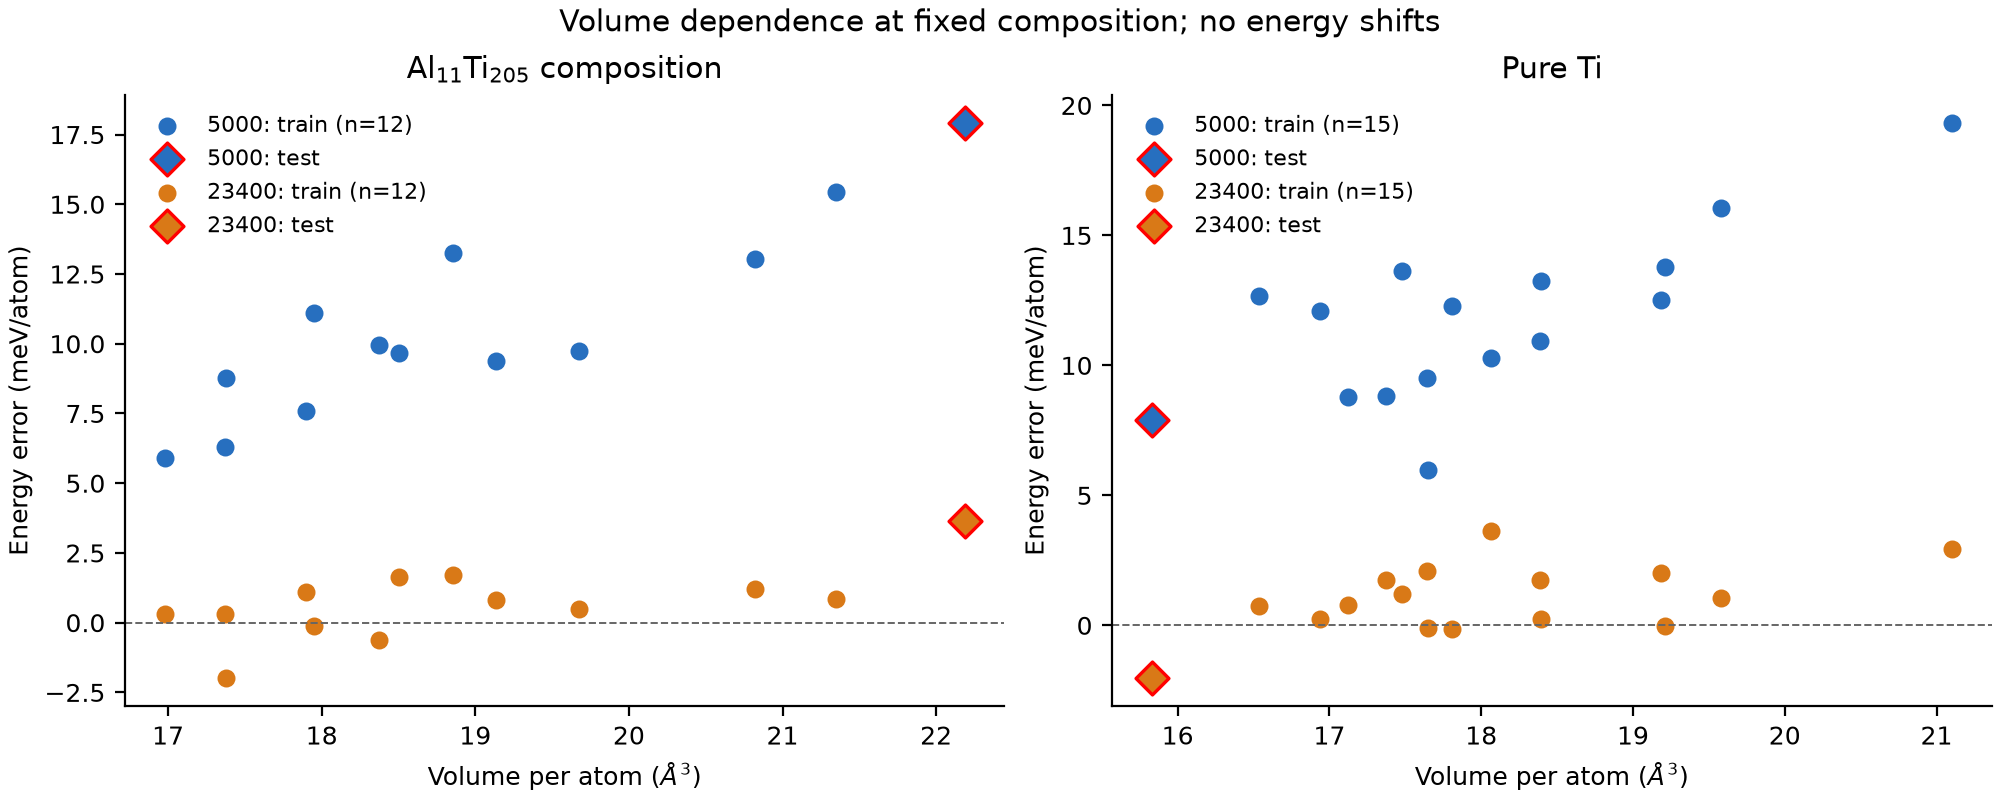
\includegraphics[width=\linewidth]{figures/supporting/fixed_composition_volume.png}
\caption{Energy residuals at fixed composition for 5k and 23.4k. Circles are training configurations; outlined diamonds are the corresponding held-out structures. The Al$_{11}$Ti$_{205}$ test structure is TiAl-test-009. The reduction on training and test structures shows that the 5k bias cannot be explained by the single largest test residual.}
\label{fig:volume}
\end{figure}

\begin{figure}[htbp]
\centering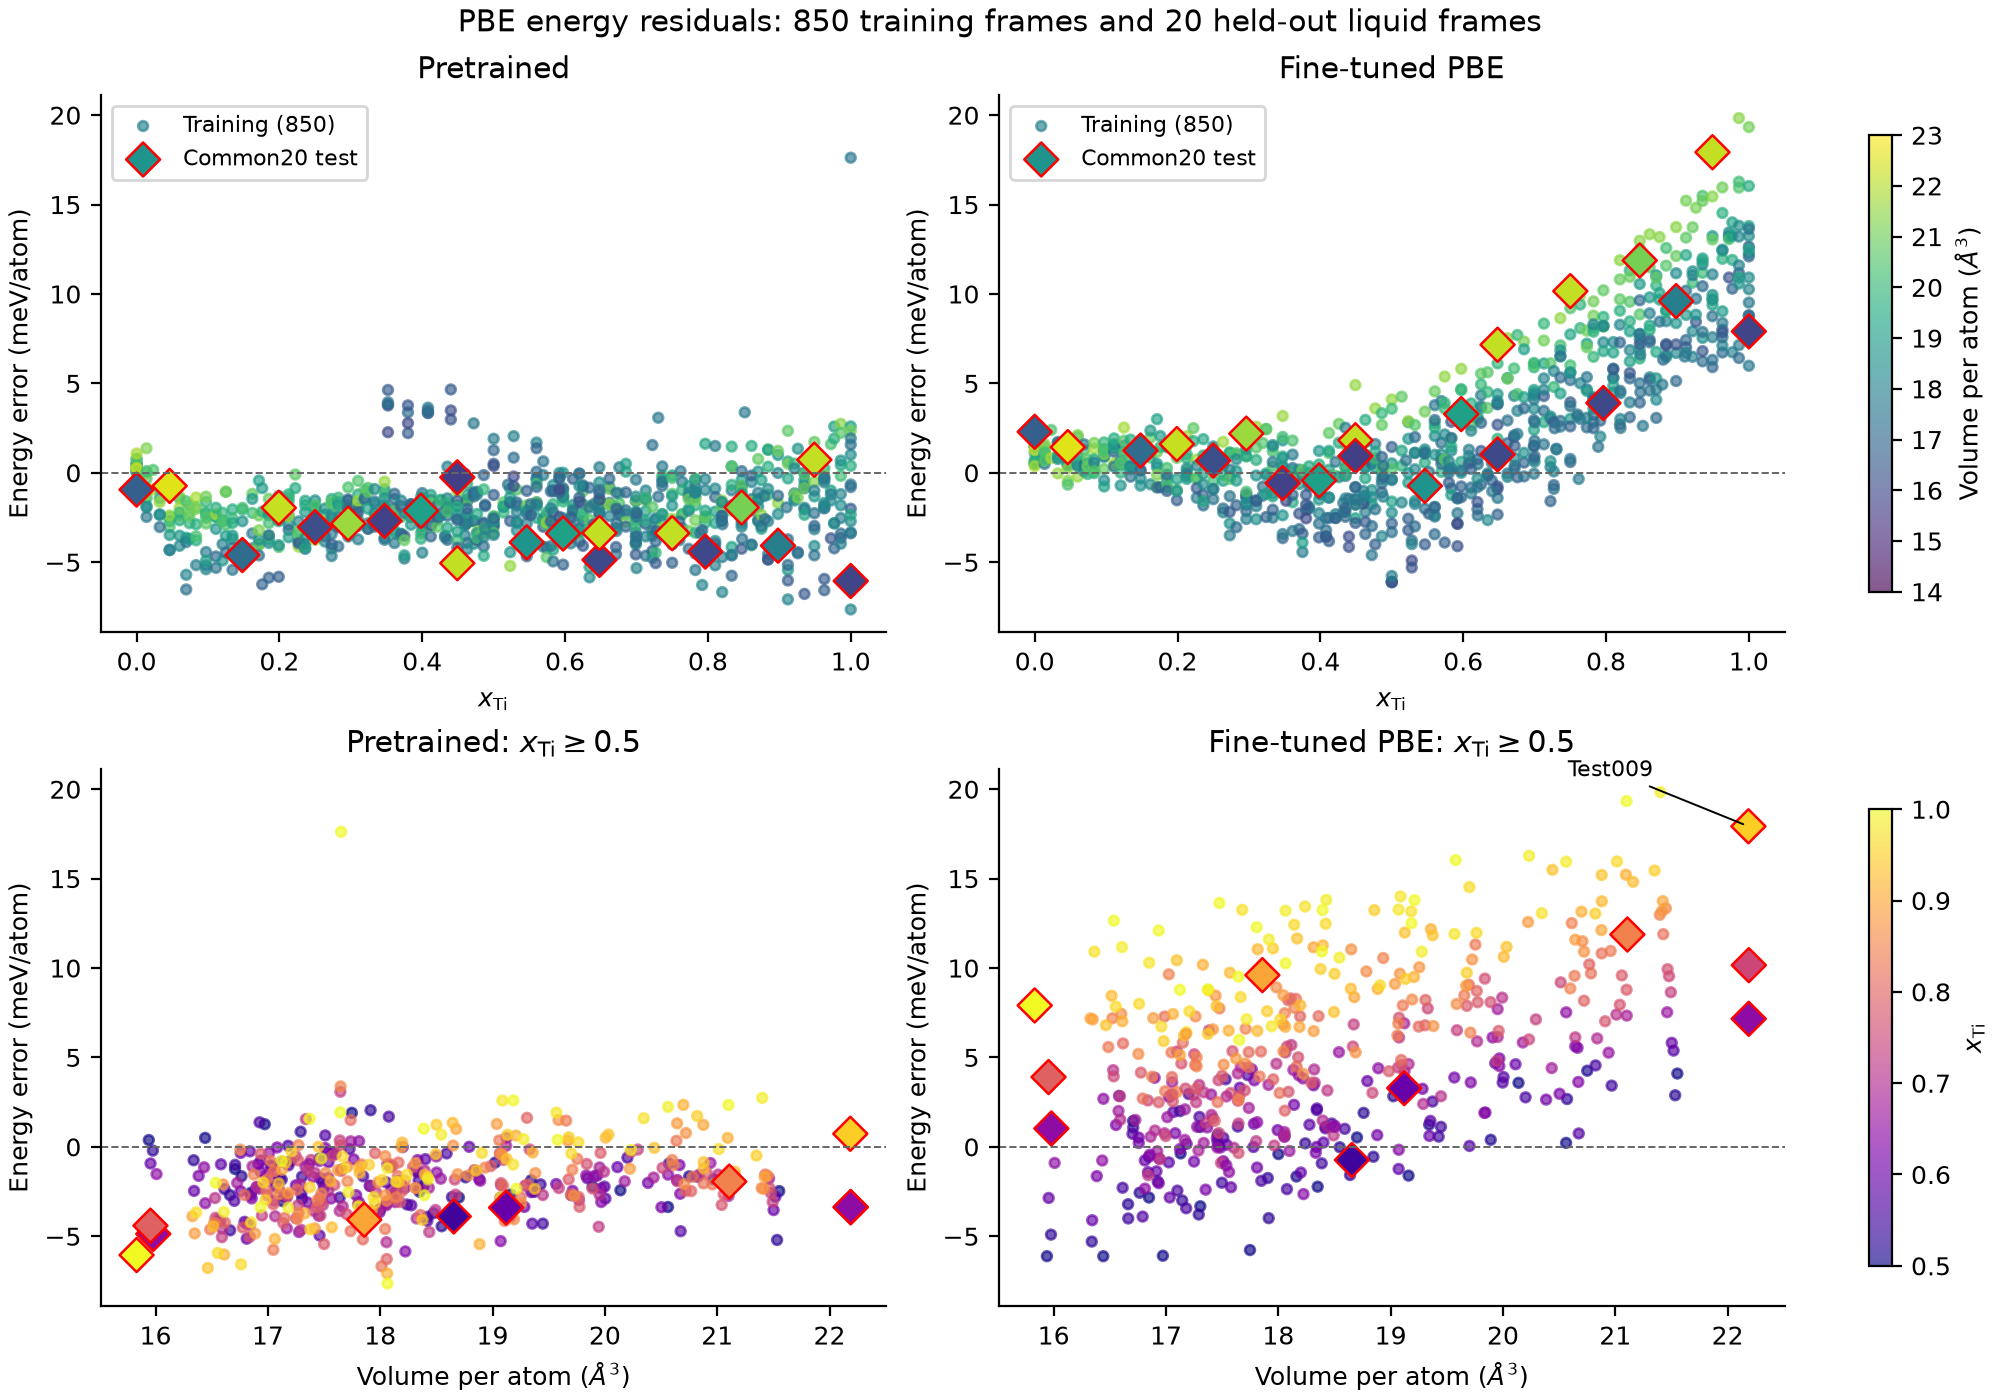
\includegraphics[width=.96\linewidth]{figures/supporting/train_test_residuals.png}
\caption{Original pretrained-versus-5k energy diagnostic on the PBE training configurations and common liquid test subset. The top panels show composition dependence with color indicating atomic volume; the bottom panels show volume dependence for $x_{\rm Ti}\geq0.5$ with color indicating composition. The continued-training comparison is given in Figs.~\ref{fig:sweep} and \ref{fig:volume}. Training-set trends are fitting diagnostics, not independent generalization estimates.}
\label{fig:original_bias}
\end{figure}

\section{Harmonic phonons: separating checkpoint and geometry effects}
\label{sec:phonons}
This section documents the earlier ASE checkpoint-selection study. Its independently optimized cells and supercells differ from the matched Phonopy calculations used in the current main-text Fig.~2 (Sec.~\ref{sec:matched_phonons}).
\subsection{Common and separately optimized hcp cells}
The 5k, 20k, and 23.4k models were compared first at the archived hcp-Ti geometry used for the original 5k model, and then at each model's own equilibrium cell. The archived calculation relaxed volume at fixed $c/a$. In the new equilibrium calculations, $a$ and $c$ were optimized independently at zero external stress, preserving hcp fractional coordinates. Residual stress components were below $3\times10^{-5}$~GPa, and the curvature with respect to $a,c$ deformations was positive. Energies and stresses of the two-atom cell were checked against its $4\times4\times4$ replication. Table~\ref{tab:cells} distinguishes these geometries from the DFT reference cell used in Sec.~\ref{sec:dos}.

\begin{table}[htbp]
\centering
\caption{hcp-Ti cells used in the checkpoint analysis. Lattice parameters are in \AA{} and atomic volumes in \AA$^3$. ``DFT reference'' identifies the supplied DFT geometry; no claim of zero MLIP stress is implied.}
\label{tab:cells}
\begin{tabular}{lrrrr}
\toprule
Geometry & $a$ & $c$ & $c/a$ & $V/N$\\
\midrule
Common archived & 2.934990 & 4.639684 & 1.580817 & 17.306227\\
Own 5k & 2.934643 & 4.640715 & 1.581356 & 17.305972\\
Own 20k & 2.938187 & 4.637391 & 1.578317 & 17.335371\\
Own 23.4k & 2.937550 & 4.638801 & 1.579139 & 17.333126\\
15k equilibrium & 2.938057 & 4.635747 & 1.577827 & 17.327694\\
DFT reference & 2.950000 & 4.680000 & 1.586441 & 17.635611\\
\bottomrule
\end{tabular}
\end{table}

All new MLIP phonons were obtained by native CPU force evaluations with central finite displacements of $\pm0.01$~\AA{} and a Ti mass of 47.867~amu. The two-atom primitive cell requires 12 displaced force evaluations plus the undisplaced reference. Force constants were treated with the ASE Frederiksen correction, three symmetrization iterations, and the acoustic sum rule; uncorrected force constants were retained for diagnostics. Final comparisons use $9\times9\times9$ supercells (1458 atoms). The path $\Gamma$--K--M--$\Gamma$--A contains 200 common reduced wave vectors; plots use the path coordinate of the common cell. Differences compare frequency-ordered eigenvalues, without tracking polarization through crossings.

Changing checkpoint has a much larger effect than relaxing each model's cell relative to the common archived geometry (Fig.~\ref{fig:bands}). At fixed geometry, the 20k-minus-5k and 23.4k-minus-5k frequency differences have RMS values 0.1211 and 0.1290~THz, with maximum absolute differences 0.3639 and 0.4372~THz. The RMS changes induced by separate relaxation are only 0.00269, 0.01090, and 0.00824~THz for 5k, 20k, and 23.4k. At their own cells, the upper optical frequency at $\Gamma$ decreases from 5.476 to 5.122 and 5.040~THz. The checkpoint effect therefore reflects changes in local force constants, not primarily changes in equilibrium lattice parameters.

\begin{figure}[htbp]
\centering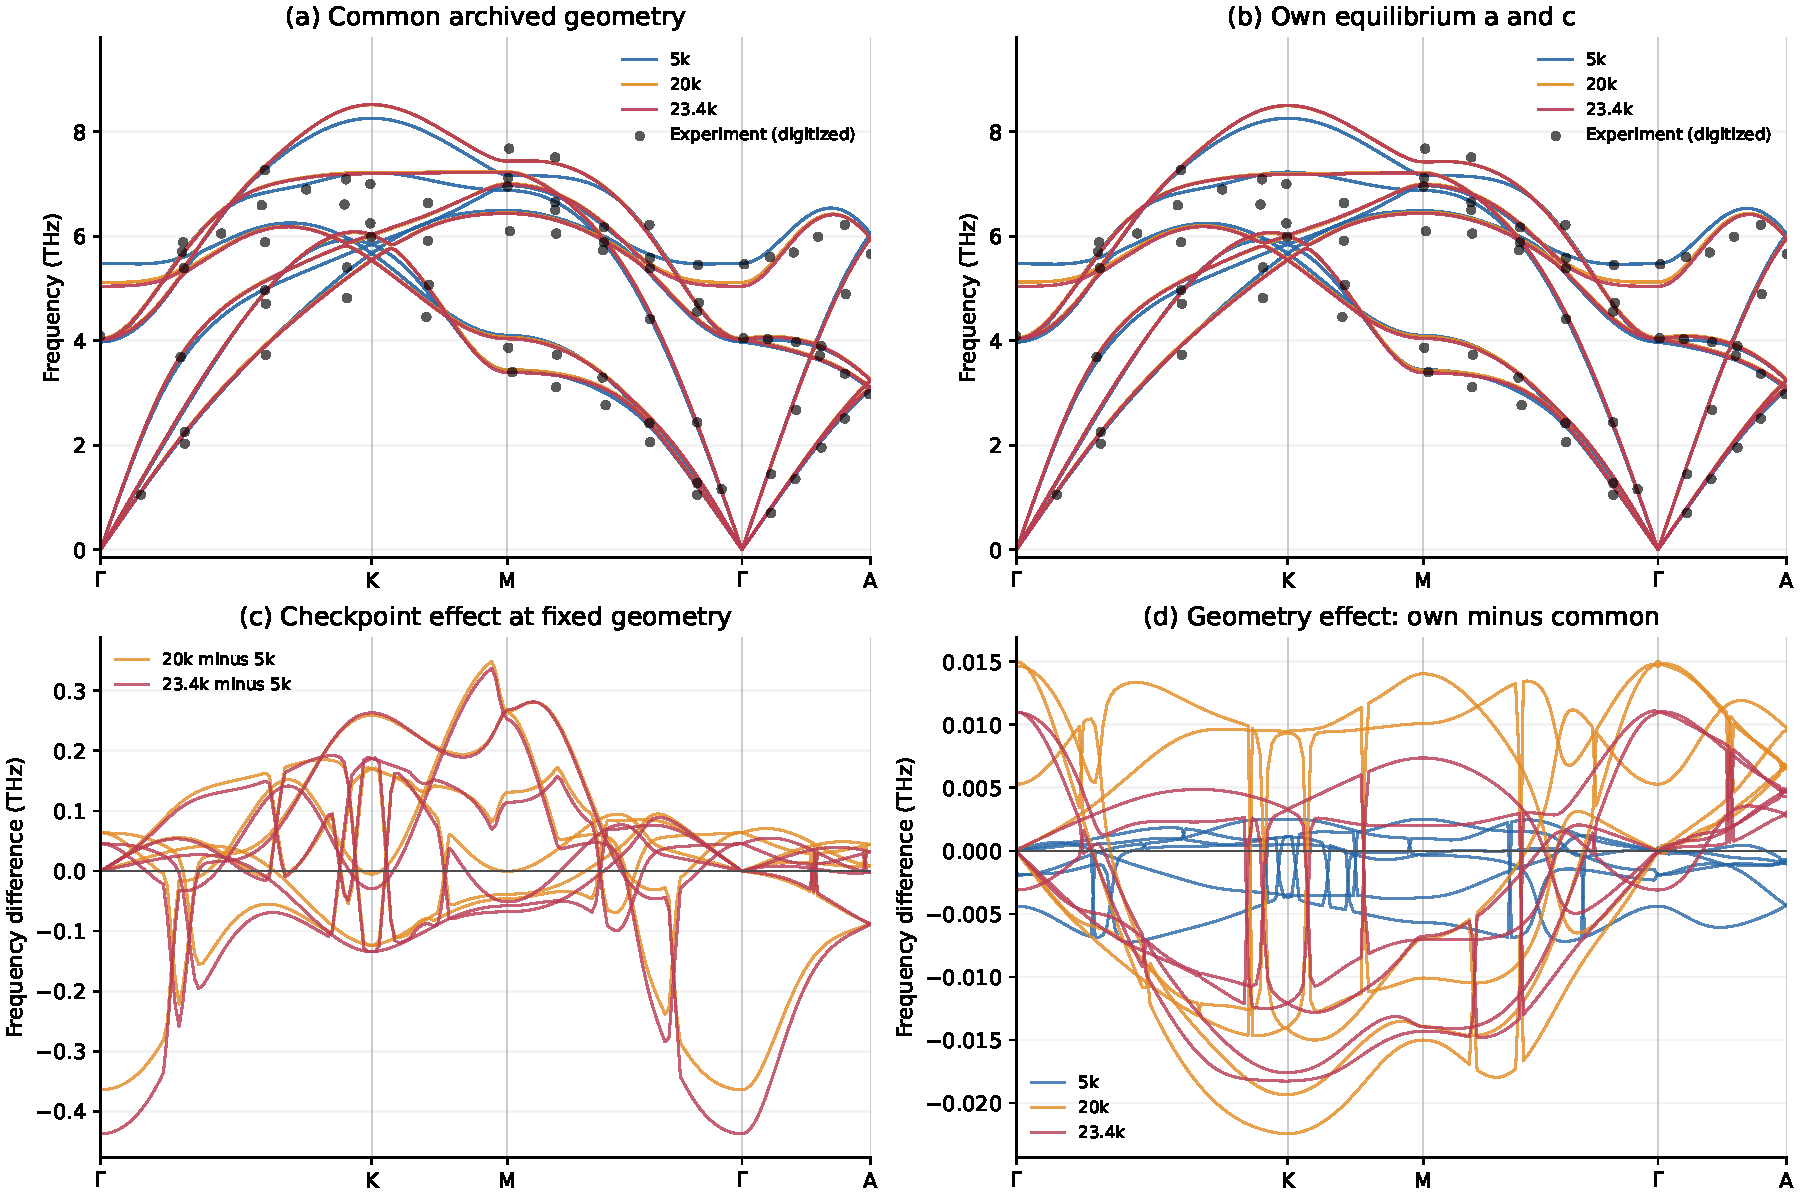
\includegraphics[width=.96\linewidth]{figures/supporting/checkpoint_phonons.pdf}
\caption{hcp-Ti dispersions at (a) the common archived geometry and (b) each model's equilibrium $a,c$. Panels (c) and (d) separate checkpoint and geometry effects. All curves use $9^3$ supercells and identical reduced wave vectors. Experimental points are the room-temperature data reproduced by Souvatzis \textit{et al.}\cite{Souvatzis2007}; they are shown as a secondary comparison and were not the checkpoint-selection criterion. Differences near crossings are between sorted frequencies, not tracked mode polarizations.}
\label{fig:bands}
\end{figure}

\subsection{Numerical checks and comparison with experimental dispersions}
The archived 5k spectrum is reproduced at its original $5^3$ supercell and geometry within 0.000332~THz maximum absolute difference. Reducing the displacement from 0.01 to 0.005~\AA{} at $5^3$ changes frequencies by at most 0.00228~THz across the six model/geometry cases. Increasing the supercell from $5^3$ to $7^3$ changes individual frequencies by up to 0.2447~THz; increasing it from $7^3$ to $9^3$ changes them by up to 0.0830~THz, with RMS changes 0.0071--0.0109~THz. Consequently, complete convergence of absolute frequencies beyond $9^3$ is not established.

The quantities of interest are more stable than those absolute frequencies. Increasing $7^3$ to $9^3$ changes the \emph{checkpoint differences} by only 0.0052--0.0056~THz RMS and the \emph{geometry-induced differences} by less than 0.00047~THz RMS. The final calculations show no imaginary frequencies below $-0.01$~THz on the sampled path or DOS mesh; the tiny negative acoustic values at $\Gamma$ are below 0.0005~THz in magnitude. These checks support the comparative interpretation, while retaining a finite-supercell limitation.

The 77 digitized room-temperature experimental points have no branch labels or pointwise uncertainties. A descriptive distance to the nearest calculated frequency branch gives RMS values 0.2201, 0.2030, and 0.1992~THz for 5k, 20k, and 23.4k at their own cells. This statistic does not favor 5k overall, although individual branches can do so. It is not a validated branch-resolved error metric, and the harmonic calculations do not include finite-temperature renormalization. This comparison must therefore be distinguished from the actual selection criterion, the DFT DOS. Figure~\ref{fig:mlip_dos} shows the corresponding redistribution of harmonic spectral weight.

\begin{figure}[htbp]
\centering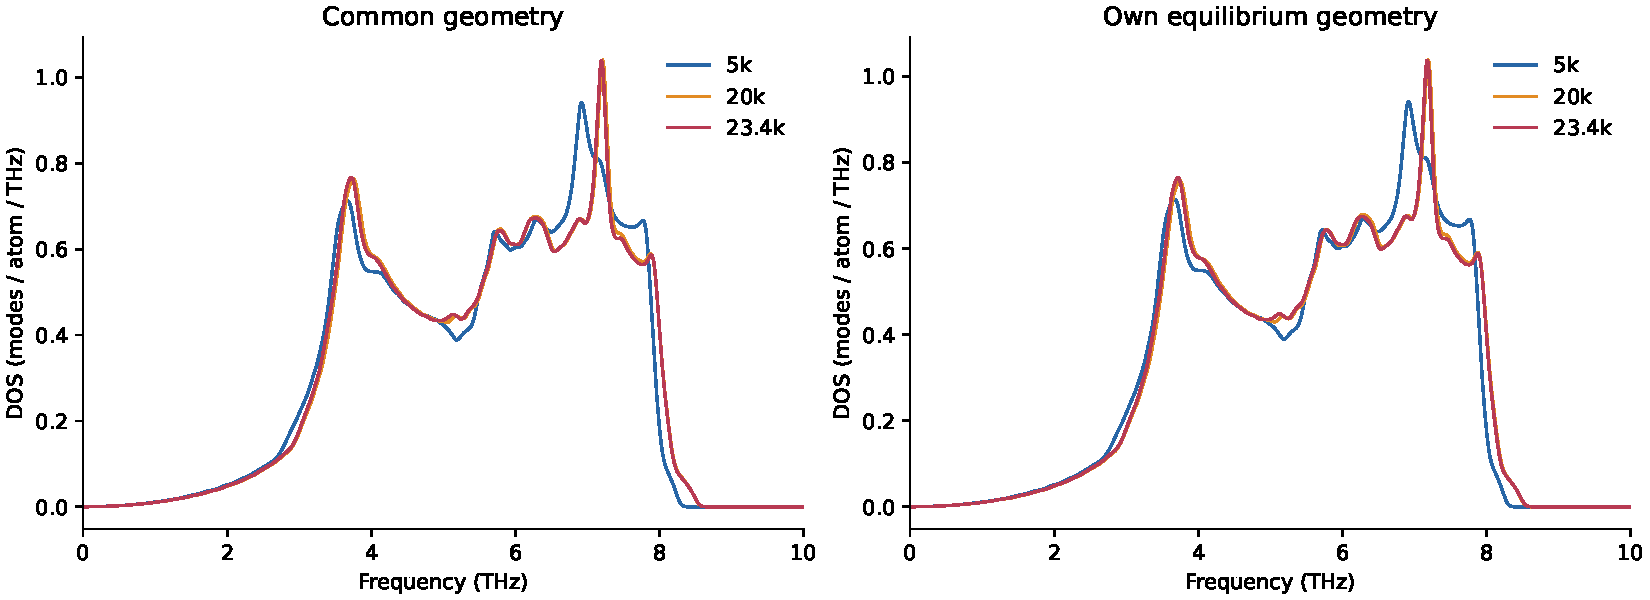
\includegraphics[width=\linewidth]{figures/supporting/checkpoint_phonon_dos.pdf}
\caption{MLIP DOS at common and separately optimized cells, using $9^3$ supercells, a $50^3$ Monkhorst--Pack mesh, Gaussian width 0.04836~THz, and normalization to three modes per atom. This figure compares checkpoints without a DFT reference. The DFT comparisons below use a common broadening of 0.05~THz.}
\label{fig:mlip_dos}
\end{figure}

\section{Comparison with the archived PBE DFT phonon DOS}
This archived PBE-only comparison was used for checkpoint selection. It is separate from the new three-functional DFT references in main-text Fig.~2 and Sec.~\ref{sec:matched_phonons}.
\label{sec:dos}
\subsection{Reference and spectral metrics}
The independent PBE DFT reference is the archived hcp-Ti calculation supplied with this project. Its unit cell has $a=2.950$~\AA, $c=4.680$~\AA, and volume 17.63561~\AA$^3$/atom. The DFT force calculations used a $4\times4\times3$ supercell (96 atoms), a 500~eV plane-wave cutoff, a $4\times4\times4$ electronic $k$-point mesh, smearing width 0.2~eV, and electronic tolerance $10^{-8}$~eV. The archived DOS used a $40\times40\times30$ phonon mesh and Gaussian width 0.05~THz, with a frequency spacing of 0.01~THz. Its integral of six modes per primitive cell was converted to three modes per atom. The original mesh file is unavailable, so the phonon-mesh centering was explicitly tested in the MLIP comparison.

All spectra below have the same normalization and broadening; no frequency shift or rescaling is fitted. For a DOS $g(\nu)$ and reference $g_{\rm DFT}(\nu)$, we use
\begin{align}
L_2^{\rm rel} &= \left[\frac{\int [g(\nu)-g_{\rm DFT}(\nu)]^2\,d\nu}{\int g_{\rm DFT}(\nu)^2\,d\nu}\right]^{1/2},\\
D_{\rm TV} &= \frac12\int |p(\nu)-p_{\rm DFT}(\nu)|\,d\nu,\\
W_1 &= \int |P(\nu)-P_{\rm DFT}(\nu)|\,d\nu,
\end{align}
where $p=g/3$ and $P$ is its cumulative integral. The first two quantities are dimensionless and $W_1$ is in THz. They describe spectral-shape differences, not statistical significance or experimental accuracy.

\subsection{Initial comparison at MLIP geometries}
Within the initial comparison restricted to 5k, 20k, and 23.4k, 5k is closer to the DFT DOS at both the common archived cell and each model's own equilibrium cell (Fig.~\ref{fig:old_dft}). For the own-cell comparison, $L_2^{\rm rel}$ is 0.3133, 0.3750, and 0.3686, respectively. The corresponding $D_{\rm TV}$ values are 0.1325, 0.1655, and 0.1625, and $W_1$ values are 0.2672, 0.3091, and 0.2965~THz. The principal high-frequency peak lies at approximately 6.92, 7.19, and 7.18~THz, versus 6.84~THz for DFT. The same ranking holds at Gaussian widths 0.05, 0.10, and 0.15~THz. However, these comparisons mix force-constant and geometry effects, because the DFT cell is larger than the MLIP equilibrium cells.

\begin{figure}[htbp]
\centering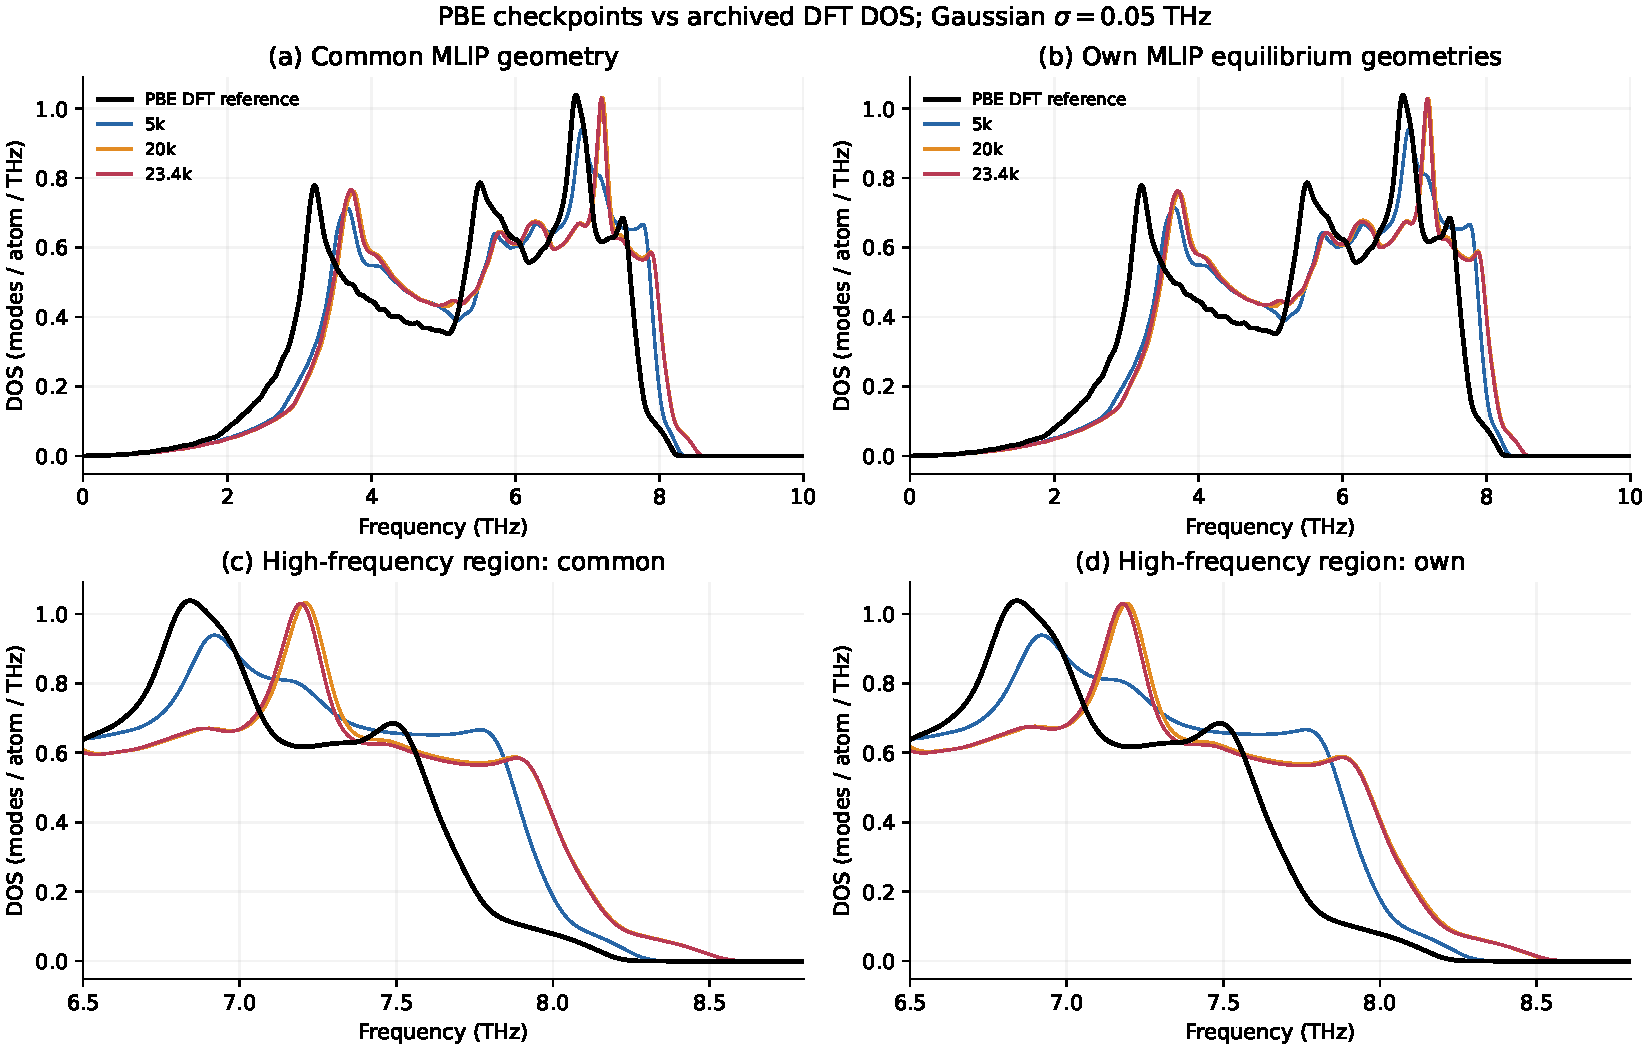
\includegraphics[width=.96\linewidth]{figures/supporting/checkpoint_dos_vs_dft.pdf}
\caption{Initial DFT-DOS comparison at the common archived and own equilibrium MLIP cells, including high-frequency detail. The DFT reference has a different cell. MLIP curves use the $50^3$ mesh and are additionally broadened from 0.04836 to 0.05~THz total Gaussian width to match the reference. This comparison motivates the identical-geometry calculation in Fig.~\ref{fig:matched_dft}.}
\label{fig:old_dft}
\end{figure}

\subsection{Five-checkpoint comparison at identical and equilibrium geometries}
All five checkpoints were evaluated at the unmodified DFT cell and fractional coordinates, without relaxation, using $9^3$ supercells, central displacements of $\pm0.01$~\AA, and the same force-constant corrections. The primary DOS comparison uses a $40\times40\times30$ Monkhorst--Pack mesh and Gaussian width 0.05~THz. Separate equilibrium calculations independently optimize $a$ and $c$ for every checkpoint.

\begin{table}[htbp]
\centering
\caption{DOS discrepancies against the PBE DFT reference for all five checkpoints. The first three metrics use exactly the DFT geometry; the last column uses each model's own equilibrium cell. All curves use the same $40\times40\times30$ mesh and 0.05~THz broadening.}
\label{tab:dos}
\begin{tabular}{lrrrr}
\toprule
Checkpoint & $L_2^{\rm rel}$ & $D_{\rm TV}$ & $W_1$ (THz) & Own-cell $L_2^{\rm rel}$\\
\midrule
5k & 0.2491 & 0.1066 & 0.1449 & 0.3134 \\
10k & 0.3415 & 0.1462 & 0.2414 & 0.4085 \\
15k & 0.1982 & 0.0826 & 0.0826 & 0.2817 \\
20k & 0.3113 & 0.1319 & 0.1915 & 0.3750 \\
23.4k & 0.3018 & 0.1274 & 0.1788 & 0.3686 \\
\bottomrule
\end{tabular}
\end{table}

\begin{figure}[htbp]
\centering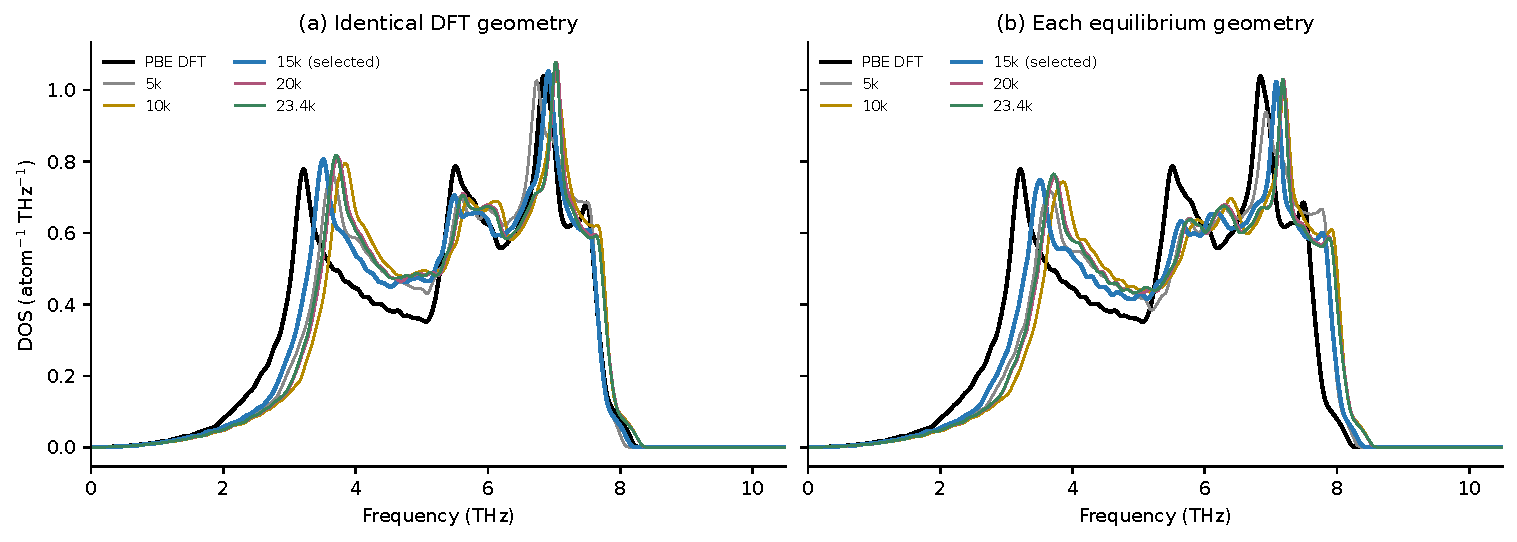
\includegraphics[width=\linewidth]{figures/supporting/dos_five_checkpoints.pdf}
\caption{The full five-checkpoint PBE comparison: (a) identical DFT geometry and (b) independently optimized equilibrium cells. The reference is the same PBE DFT DOS in both panels. All spectra integrate to three modes per atom; no frequency shift or rescaling is applied. The selected 15k curve has the smallest integral discrepancy in both comparisons.}
\label{fig:matched_dft}
\end{figure}

At identical DFT geometry, 15k reduces $L_2^{\rm rel}$ from 0.2491 to 0.1982 relative to 5k, a 20\% reduction. The total-variation and Wasserstein discrepancies decrease by approximately 22\% and 43\%, respectively. Its preference is preserved for all three metrics on the tested $40\times40\times30$ and $50^3$ Monkhorst--Pack meshes and the $\Gamma$-centered $40\times40\times30$ mesh, at Gaussian widths of 0.05, 0.10, and 0.15~THz. The ordering at fixed geometry is 15k, 5k, 23.4k, 20k, and 10k. The evolution with training is therefore nonmonotonic.

After independent relaxation, the 15k cell has $a=2.938057$~\AA, $c=4.635747$~\AA, and $V/N=17.327694$~\AA$^3$. Its relative DOS discrepancy is 0.2817, versus 0.3134 for 5k, retaining an approximately 10\% advantage. This integral improvement does not imply improvement of every peak: the principal own-cell peaks are about 7.08~THz for 15k and 6.92~THz for 5k, compared with 6.84~THz for DFT. The selected 15k optical frequencies at $\Gamma$ are 3.8196, 3.8204, and 4.9962~THz; its maximum on the sampled path is 8.3378~THz.

\begin{figure}[htbp]
\centering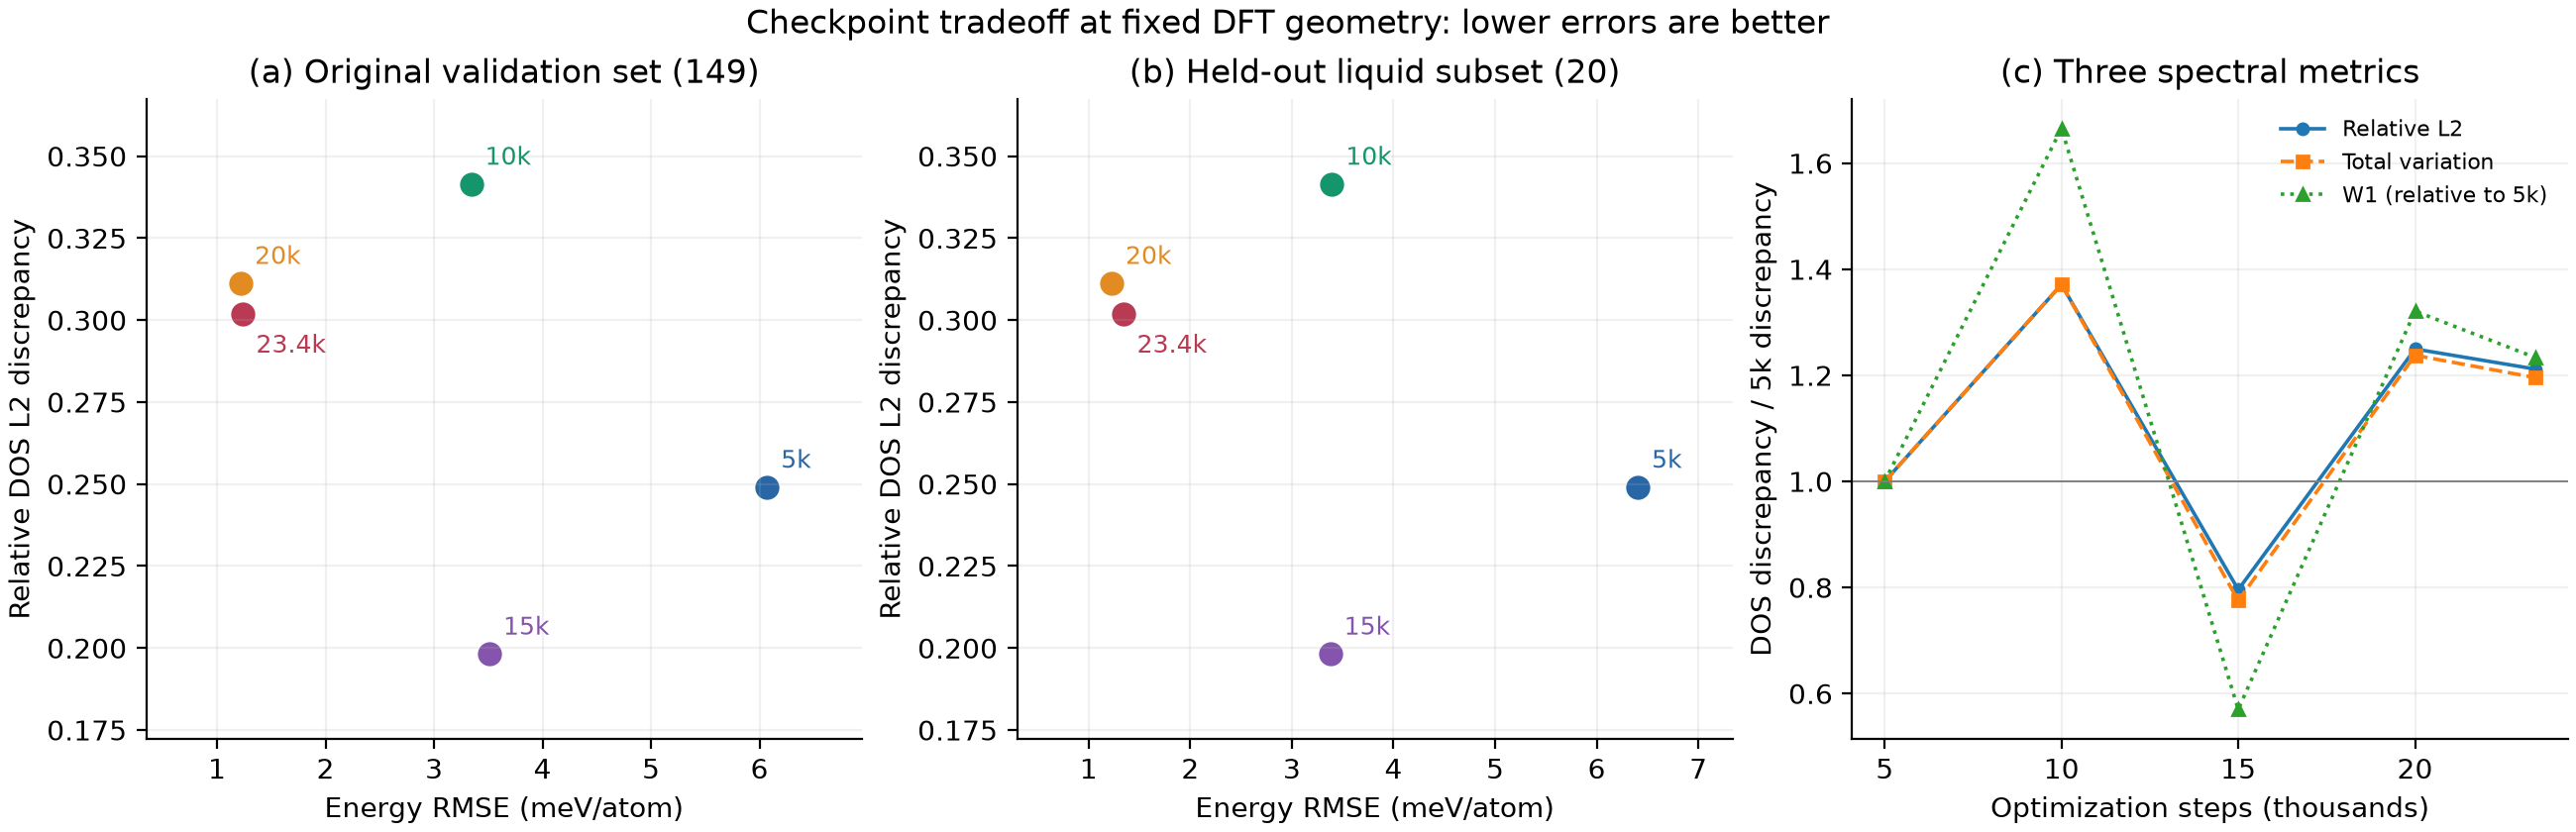
\includegraphics[width=.92\linewidth]{figures/supporting/checkpoint_tradeoff.png}
\caption{Tradeoff between the fixed-geometry DFT-DOS discrepancy and complete validation/test energy RMSEs for the five PBE checkpoints. The test panel uses the original fixed 20-structure liquid diagnostic subset. The selected 15k model minimizes the DOS discrepancy; 20k and 23.4k have smaller energy errors.}
\label{fig:tradeoff}
\end{figure}

\subsection{Numerical limitations}
Identical geometry removes an important confounder but does not make the DFT and MLIP numerical protocols identical. DFT uses a $4\times4\times3$ force-constant supercell whereas the final MLIP comparison uses $9^3$. The original 5k/20k/23.4k size checks support the stability of checkpoint differences but do not establish full convergence of every absolute frequency, nor a separate size-convergence result for 15k. The selected 15k spectrum has no imaginary frequencies below $-0.01$~THz on the sampled path; the largest acoustic residual at $\Gamma$ is about $-0.00027$~THz. This archived PBE DFT DOS is not a same-functional reference for PBEsol or \rscan{}; the new matched comparison supplies a separate DFT reference for each functional.


\section{Current benchmark and checkpoint coverage}
The test design comprises 50 geometries selected before evaluating model errors. The present numerical snapshot contains 30 completed common DFT triplets: TiAl-test-001--020, -026--029, -034--036, and -043--045. These comprise 20 liquid-pool, four hcp, three bcc, and three $\gamma$-TiAl source structures, with 20\,532 force components. The main-text captions and metric table state the actual sample size; no predictions or labels for the remaining structures are imputed.

The PBE benchmark now uses 20k, while the main physical-property results retain the allocation in Table~\ref{tab:coverage}. PBEsol and \rscan{} retain their frozen exports, and the pretrained predictions are unchanged. Energies are raw, without fitted offsets. PBE 20k energy MAE/RMSE is 1.138/1.514~meV/atom, force MAE/RMSE is 0.04694/0.06376~eV/\AA, and stress MAE/RMSE is 0.05465/0.08205~GPa. Full metrics and bootstrap intervals are in \texttt{test30\_metrics.json}. All 36 energy/force/stress MAE and RMSE entries for fine-tuned and pretrained models were independently reproduced from the cached predictions and checked model/geometry hashes.

The change to 20k followed inspection of Test50 results and does not constitute blind selection. No model weights or energy offsets were fitted to the holdout, but the reported comparisons are conditional on retrospective model selection, the completed geometries, and unknown trajectory correlations. The 20-structure checkpoint sweep elsewhere in this document is preserved as its original diagnostic and must not be confused with the 30-structure benchmark.

\begin{table}[htbp]
\centering
\caption{PBE checkpoint coverage in the current revision. PBEsol and \rscan{} retain their final checkpoints throughout.}
\label{tab:coverage}
\begin{tabular}{p{.68\linewidth}l}
\toprule
Result & PBE checkpoint\\
\midrule
Current 30-structure parity plots and MAE/RMSE & 20k\\
$\alpha$-Ti dispersion and DOS & 15k\\
Mixing enthalpy at 2000~K, all 11 compositions & 15k\\
Density and excess volume at 1873~K, all 11 compositions & 15k\\
Ti density: solids 300--1900~K and liquids 1873--2500~K & 15k\\
Ti solid--liquid coexistence and melting estimate & 15k\\
Pure-Ti viscosity at 1873 and 2000~K & 15k\\
Alloy viscosity at 1873~K, $x_{\rm Al}=0.20,0.45,0.80$ & 15k\\
Original Ti temperature-dependent density series & 5k, retained for comparison\\
Ti$_3$Al harmonic phonons & 5k, retained\\
\bottomrule
\end{tabular}
\end{table}

Checkpoint allocation is stated in the main Fine-tuning subsection; subsequent main-text sections and figures use the functional label PBE. This convention does not reassign historical data to another model. All PBE viscosities shown in the main article now use 15k; the older 5k alloy and pure-Ti transport points are excluded. Historical TDM and checkpoint diagnostics retain their original identities.

\section{Updated PBE mixing enthalpy at 2000 K}
All 11 compositions were simulated with 15k in 200-atom cells at a nominal 2000~K and external pressure of 1~bar, using a 1~fs step and the same Melchionna NPT settings as the earlier liquid workflow. Each run starts from the final archived 5k liquid configuration and includes 30~ps equilibration followed by 30~ps production. Velocities and the NPT integrator are restarted between these stages. Energies, temperature, pressure, volume, density, and enthalpy are logged every 10~fs; configurations are saved every 100~fs. The pure-Ti 2000~K density from this production stage is shown alongside the corresponding 5k point in the main-text temperature plot; the full 2000~K composition-dependent density curve remains a supporting diagnostic.

Enthalpy is evaluated as $H_m=N_{\rm A}\langle E_{\rm pot}+E_{\rm kin}+p_{\rm ext}V\rangle/N$, with a positive external-pressure term and each checkpoint's own pure-liquid references. The main estimate uses only the complete 30~ps production stage. A trajectory mean's standard error is the maximum block SEM over 3, 5, and 6~ps blocks, with at least four blocks. Independent-trajectory propagation includes the mixture and both pure components; shared endpoint references correlate different compositions. These errors describe finite sampling within one trajectory per state and exclude model error, finite-size effects, and between-replica variability.

\begin{table}[htbp]
\centering
\caption{Updated PBE 15k mixing enthalpy at 2000~K in kJ/mol of atoms, using 30~ps production. Endpoint values vanish by definition.}
\label{tab:enthalpy}
\begin{tabular}{rrr}
\toprule
$x_{\rm Al}$ & $\Delta H_{\rm mix}$ & SEM\\
\midrule
0.0 & 0.000 & 0.000 \\
0.1 & -7.152 & 0.162 \\
0.2 & -13.713 & 0.147 \\
0.3 & -18.711 & 0.165 \\
0.4 & -22.747 & 0.182 \\
0.5 & -25.007 & 0.302 \\
0.6 & -23.914 & 0.210 \\
0.7 & -21.163 & 0.249 \\
0.8 & -15.466 & 0.150 \\
0.9 & -8.036 & 0.157 \\
1.0 & 0.000 & 0.000 \\
\bottomrule
\end{tabular}
\end{table}

The equiatomic minimum is $-25.007\pm0.302$~kJ/mol, compared with $-26.284\pm0.263$~kJ/mol in the reprocessed 5k archive. The 15k curve is less exothermic over the interior compositions. Its equal-weight mean absolute discrepancy against the same nine provisional calorimetric points used in the main article is 3.61~kJ/mol, compared with approximately 3.1~kJ/mol for PBEsol and 1.47~kJ/mol for the current 60~ps \rscan{} series. The comparison therefore preserves the overall enthalpy ranking in favor of \rscan{}, while increasing the PBE discrepancy. It does not motivate selecting a checkpoint by agreement with the calorimetric curve.

\begin{figure}[htbp]
\centering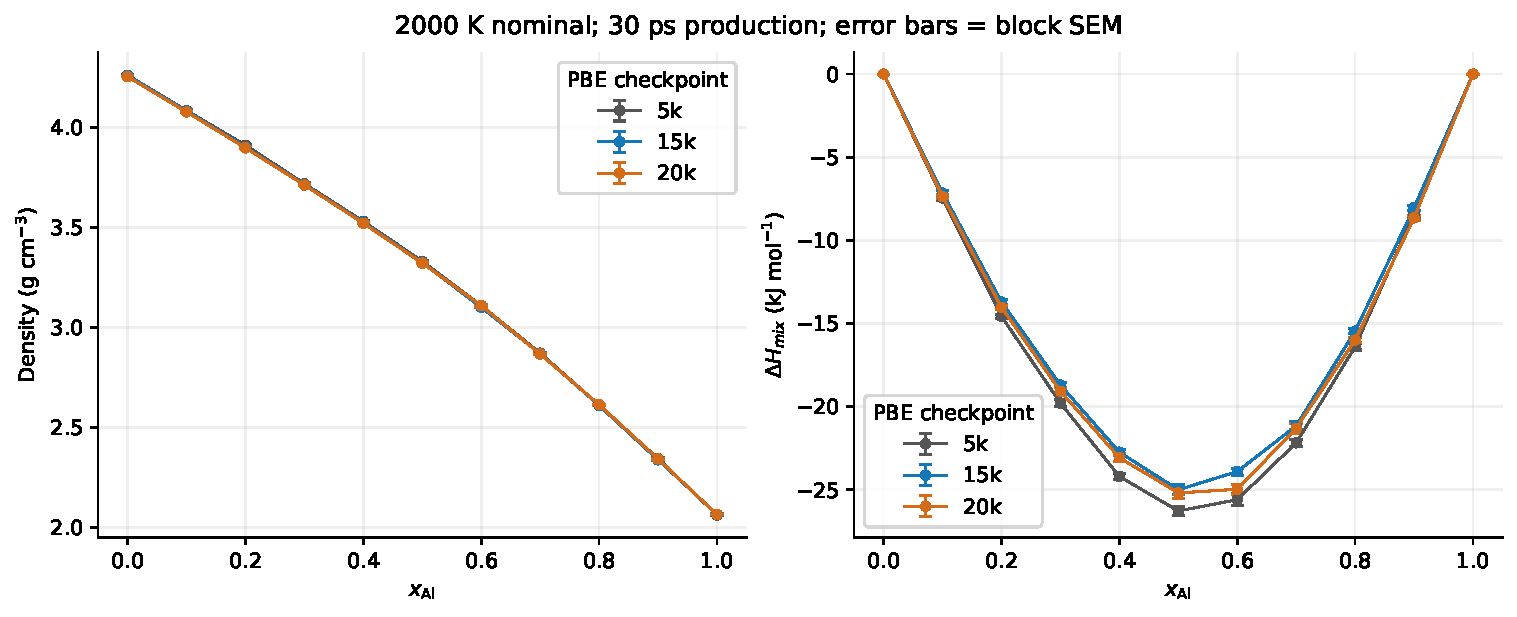
\includegraphics[width=\linewidth]{figures/supporting/density_enthalpy_5k_15k_20k.pdf}
\caption{Completed 2000~K checkpoint comparison using 30~ps production: density and enthalpy of mixing for PBE 5k, 15k, and 20k. The updated main-text enthalpy uses 15k. The full density comparison is a supporting diagnostic; its 15k pure-Ti endpoint also supplies the updated 2000~K point in the main-text temperature plot.}
\label{fig:enthalpy_checkpoints}
\end{figure}

\subsection{Sensitivity to equilibration and sampling}
An extended window combines 10--30~ps of equilibration with 1--30~ps of production, yielding 49~ps. The first production picosecond is excluded because velocities and the thermostat/barostat were restarted. Blocks do not cross this restart, and stage means are weighted by duration. This expansion changes the 15k mixing enthalpy by at most 0.35~kJ/mol and leaves the broad difference from 5k intact. Individual windows show fluctuations and possible drift, so the 49~ps estimate is a sensitivity check rather than the primary result. The full audit retains other cutoffs and block lengths.

\begin{figure}[htbp]
\centering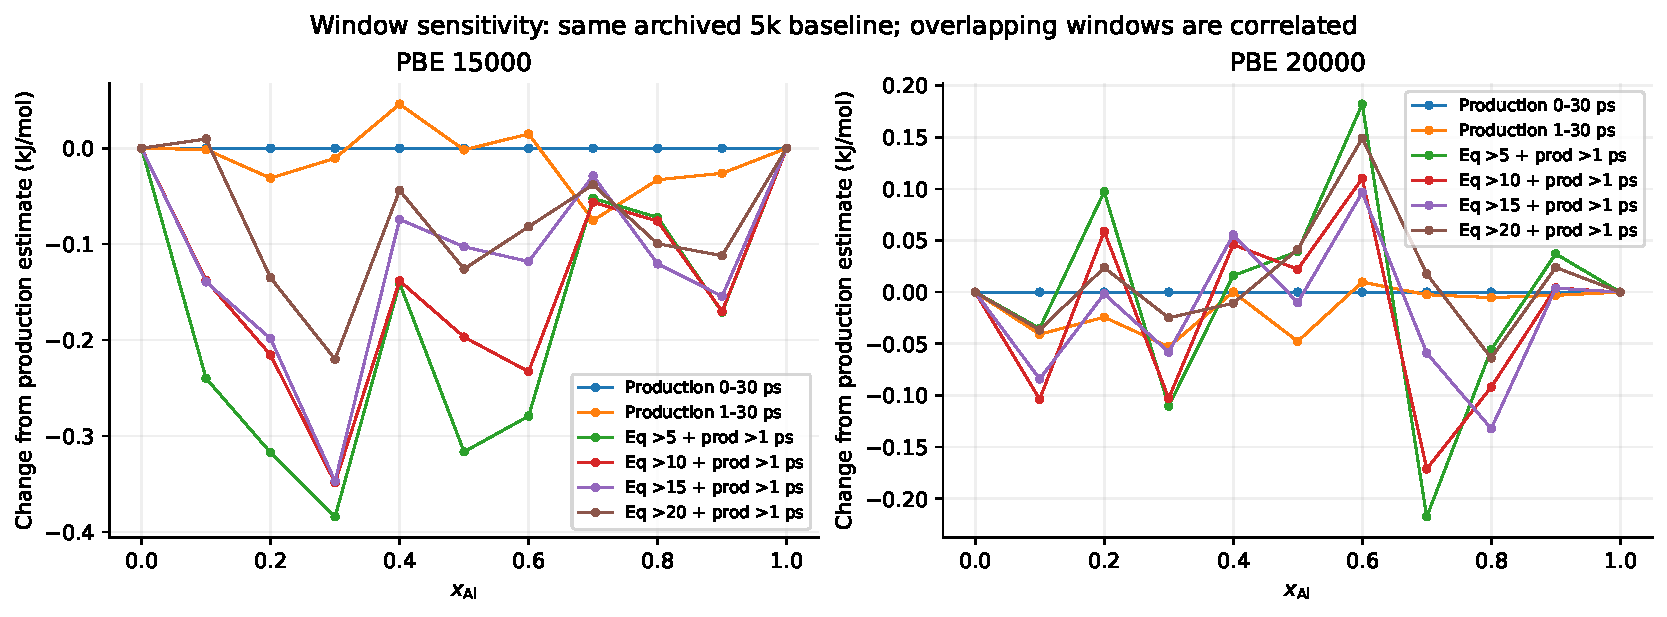
\includegraphics[width=\linewidth]{figures/supporting/equilibration_window_sensitivity.pdf}
\caption{Sensitivity to including late equilibration in the sampling window. Extended windows exclude the first picosecond following the velocity/integrator restart. The curves share portions of the same trajectories and are not independent estimates.}
\label{fig:window}
\end{figure}

For 200 atoms, the integrator targets $3(N-1)k_{\rm B}T/2$ whereas the logged temperature divides kinetic energy by $3N$; nominal 2000~K therefore corresponds to about 1990~K in this output. The new dense logs give 1989.91--1990.13~K. Subsampling at the older 100~fs cadence produces larger apparent temperature deviations, so the older sparse kinetic averages should not be interpreted as full-trajectory temperatures. The potential-energy mixing comparison confirms the direction of the checkpoint shift independently of this kinetic sampling effect. Diffusive motion is present in all new production trajectories. The trajectory means, block analyses, windows, and quality checks are preserved in \texttt{pbe\_checkpoint\_enthalpy\_statistics.json}.


\section{Extended r2SCAN mixing-enthalpy statistics}
All 11 liquid compositions at 2000~K were continued from the last saved coordinates, cell, and momenta for another 30\,000 steps of 1~fs, giving 60~ps of accumulated production per composition. The cells contain 200 atoms and the imposed pressure is 1~bar. The duplicate boundary frame was excluded, leaving 601 saved configurations in the combined mean. Thermostat and barostat variables were restarted; sensitivity to discarding the first 1, 2, or 5~ps after continuation was assessed separately.

Enthalpy uses $E_{\rm pot}+E_{\rm kin}+p_{\rm ext}V$, and each mixture uses the pure Al and Ti references sampled for the same total duration. Block standard errors use six or twelve 5~ps blocks for 30 or 60~ps, respectively, omitting the initial frame only in the block diagnostic. Pure-component variances are included in propagation and shared references correlate errors between compositions.

\begin{table}[htbp]
\centering
\caption{r2SCAN mixing enthalpy at 2000~K in kJ/mol of atoms. Uncertainties are propagated block SEM; endpoints vanish by definition.}
\label{tab:scan60}
\begin{tabular}{rrr}
\toprule
$x_{\rm Al}$ & 30~ps & 60~ps\\
\midrule
0.1 & $-8.634\pm0.237$ & $-8.665\pm0.147$ \\
0.2 & $-16.204\pm0.182$ & $-16.442\pm0.186$ \\
0.3 & $-23.824\pm0.164$ & $-23.462\pm0.174$ \\
0.4 & $-28.447\pm0.175$ & $-28.632\pm0.153$ \\
0.5 & $-32.039\pm0.171$ & $-31.655\pm0.192$ \\
0.6 & $-31.346\pm0.123$ & $-31.736\pm0.200$ \\
0.7 & $-28.146\pm0.330$ & $-28.126\pm0.212$ \\
0.8 & $-20.781\pm0.193$ & $-20.641\pm0.130$ \\
0.9 & $-11.024\pm0.139$ & $-10.955\pm0.120$ \\
\bottomrule
\end{tabular}
\end{table}

The maximum change in the mean curve is 0.390~kJ/mol. SEM decreases at five interior compositions and increases at four; doubled duration does not imply uniform error reduction. The numerical minimum is at $x_{\rm Al}=0.6$, but its difference from $x_{\rm Al}=0.5$ is $-0.081\pm0.263$~kJ/mol with shared-reference covariance included. The two sampled minima are not resolved statistically. The mean absolute discrepancy from the nine provisional calorimetric points is 1.468~kJ/mol.

The 30 and 60~ps estimates are nested and cannot be treated as independent means. Comparisons of disjoint 30~ps segments show no composition with a Benjamini--Hochberg-adjusted $q<0.05$ across nine compositions; this does not establish stationarity or independent blocks. At $x_{\rm Al}=0.6$, increasing the block length from 5 to 10~ps changes SEM from 0.200 to 0.267~kJ/mol. Omitting the first 1, 2, or 5~ps of continuation changes the mixing enthalpy by at most 0.041, 0.043, or 0.085~kJ/mol, respectively. Full diagnostics are retained in \texttt{r2scan\_enthalpy\_60ps.json}.

\section{Updated density at 1873 K}
All 11 PBE 15k runs used 200 atoms, 1~bar external pressure, 30~ps equilibration, and 30~ps production. The initial configurations came from the corresponding archived liquids. Model identity was verified by SHA-256, and CPU/GPU consistency was checked before MD. The primary density is $\langle M/V\rangle$ over $0<t\leq30$~ps of production, sampled every 10~fs. The excess molar volume uses $N_{\rm A}\langle V\rangle/N$ and the same 15k pure-component trajectories. Standard errors use the maximum block SEM for 3, 5, and 6~ps blocks and are propagated for excess volumes.

\begin{table}[htbp]
\centering
\caption{PBE 15k liquid density and excess molar volume at 1873~K. Errors are block standard errors, excluding protocol and model uncertainties.}
\label{tab:density15k}
\begin{tabular}{rrrrr}
\toprule
$x_{\rm Al}$ & $\rho$ (g/cm$^3$) & SEM & $V_m^{\rm ex}$ (cm$^3$/mol) & SEM\\
\midrule
0.0 & 4.28280 & 0.00076 & 0.00000 & 0.00000 \\
0.1 & 4.10658 & 0.00073 & -0.20181 & 0.00291 \\
0.2 & 3.93029 & 0.00070 & -0.40548 & 0.00311 \\
0.3 & 3.74251 & 0.00170 & -0.57790 & 0.00587 \\
0.4 & 3.55417 & 0.00151 & -0.74910 & 0.00596 \\
0.5 & 3.34969 & 0.00192 & -0.86611 & 0.00783 \\
0.6 & 3.14185 & 0.00328 & -0.96427 & 0.01286 \\
0.7 & 2.90467 & 0.00191 & -0.93673 & 0.00969 \\
0.8 & 2.64453 & 0.00255 & -0.77265 & 0.01330 \\
0.9 & 2.36855 & 0.00145 & -0.45351 & 0.01084 \\
1.0 & 2.09177 & 0.00141 & 0.00000 & 0.00000 \\
\bottomrule
\end{tabular}
\end{table}

The maximum change from the reprocessed 5k density is $-0.00956$~g/cm$^3$ ($-0.285\%$) at $x_{\rm Al}=0.5$. The excess-volume minimum is $-0.9643\pm0.0129$~cm$^3$/mol at $x_{\rm Al}=0.6$. Against the same tabulated experimental convention used in the main article, the density mean absolute discrepancy changes from 0.1160 to 0.1117~g/cm$^3$ (mean absolute relative discrepancy 3.376\% to 3.262\%). These small changes preserve the model ranking.

The archived 5k sampling interval was 100~fs. Decimating the new 15k logs to that cadence can shift a density mean by up to 0.0143~g/cm$^3$, exceeding the largest observed checkpoint difference; the two curves therefore do not isolate a pure checkpoint effect. The largest difference between the two production halves is 0.00588~g/cm$^3$, and using only the last 10~ps changes the mean by at most 0.00326~g/cm$^3$. All trajectories retain diffusive motion. Mean pressure is 0.00434--0.00983~GPa rather than exactly the imposed 0.0001~GPa; these residual and sampling effects are not included in the block SEM. The logged temperatures use $3N$ degrees of freedom; the thermostat convention $3(N-1)$ yields 1872.82--1873.06~K.

The pure-Ti density at 1873~K is $4.28280\pm0.00076$~g/cm$^3$. The independent 2000~K series described above gives $4.26057\pm0.00114$~g/cm$^3$. Both are shown as 15k in the main temperature plot. The subsequent 15-point scan completes the 15k thermal-density curve while retaining every archived 5k point for comparison.

\subsection{Completed temperature-dependent density scan}
The five new liquids at 2100--2500~K use 200 atoms, 30~ps equilibration, and 30~ps production, starting independently from the final 15k liquid configuration at 2000~K. The five $\alpha$ and five $\beta$ starting cells use 250 atoms and 20+30~ps, with their respective 15k static equilibrium lattice parameters. All runs use the same 1~fs, 1~bar isotropic Melchionna NPT settings, with scalar sampling every 10~fs. All 15 production windows are complete. The model and protocol identities, file hashes, scalar/trajectory consistency, temperature, pressure, drift, and mobility were checked before plotting.

Table~\ref{tab:ti_density_temperature15k} includes the two previously completed liquid points. The phase column denotes initialization. At 1900~K the $\beta$-initialized cell loses crystalline order during equilibration and is liquid throughout production: its last-10-ps fraction with $\bar q_6>0.25$ is 0.0004 and its 10~ps MSD is 30.30~\AA$^2$. At 1800~K the corresponding values are 0.9684 and 0.77~\AA$^2$, indicating retained crystalline order. This homogeneous-cell behavior is not an equilibrium melting bracket. Structural checks use 14 nearest neighbors, frames spaced by 1~ps, thresholds 0.20--0.35, and an independent correlated-bond criterion, consistently with the coexistence diagnostic.

The reported SEM is the maximum from 3, 5, and 6~ps blocks; it excludes model, finite-size, preparation, pressure-offset, and sampling-cadence effects. Mean logged pressures are included explicitly. The 5k/15k comparison is therefore descriptive rather than an isolated checkpoint-effect measurement.
\begin{table}[htbp]
\centering\small
\caption{Completed PBE 15k pure-Ti densities. The phase denotes the starting cell; $\beta^\ast$ at 1900 K melted before production. All averages use 30 ps production. SEM is a block standard error; $\bar P$ is the logged mean pressure, with a target of 0.1 MPa. MSD removes affine cell change and center-of-mass motion.}
\label{tab:ti_density_temperature15k}
\begin{tabular}{lrrrrr}
\toprule
Start & $T$ (K) & $\rho$ (g/cm$^3$) & SEM (g/cm$^3$) & $\bar P$ (MPa) & MSD$_{10\,\mathrm{ps}}$ (\AA$^2$)\\
\midrule
$\alpha$ & 300 & 4.55300 & 0.00015 & 2.03 & 0.04\\
$\alpha$ & 500 & 4.52871 & 0.00011 & 1.48 & 0.08\\
$\alpha$ & 700 & 4.50475 & 0.00019 & 2.04 & 0.12\\
$\alpha$ & 900 & 4.47952 & 0.00029 & 3.17 & 0.17\\
$\alpha$ & 1100 & 4.45456 & 0.00024 & 3.08 & 0.22\\
$\beta$ & 1200 & 4.44759 & 0.00027 & 4.12 & 0.38\\
$\beta$ & 1400 & 4.42088 & 0.00052 & 3.71 & 0.45\\
$\beta$ & 1600 & 4.39353 & 0.00040 & 6.10 & 0.49\\
$\beta$ & 1800 & 4.36322 & 0.00105 & 4.55 & 0.77\\
Liquid & 1873 & 4.28280 & 0.00076 & 9.83 & 29.38\\
$\beta^\ast$ & 1900 & 4.27527 & 0.00111 & 5.04 & 30.30\\
Liquid & 2000 & 4.26057 & 0.00114 & 5.29 & 36.00\\
Liquid & 2100 & 4.24152 & 0.00123 & 8.11 & 44.33\\
Liquid & 2200 & 4.22469 & 0.00108 & 9.71 & 46.19\\
Liquid & 2300 & 4.20641 & 0.00086 & 8.23 & 46.54\\
Liquid & 2400 & 4.18991 & 0.00083 & 8.45 & 53.53\\
Liquid & 2500 & 4.17173 & 0.00152 & 8.25 & 60.19\\
\bottomrule
\end{tabular}
\end{table}


\subsection{Extended liquid-Ti density for PBEsol and r2SCAN}
\label{sec:xc_liquid_density_extended}
The PBEsol 23\,100-step and \rscan{} 23\,200-step models were used, with SHA-256 prefixes \texttt{5a5359a7\allowbreak13848d98} and \texttt{8b2c339b\allowbreak f472564a}, respectively. All 14 points were completed in a single allocation on one A100. Each uses 200 Ti atoms and the final archived liquid configuration at the same temperature and functional. After 10~ps re-equilibration, 90~ps of new production is accumulated with a 1~fs step, a nominal pressure of 1~bar, isotropic Melchionna NPT, a 25~fs thermostat time parameter, and a barostat parameter $B\tau^2$ with $B=110$~GPa. Velocities and integrator variables restart at each stage, so this is not an exact continuation of the archived trajectory.

Density is $\langle M/V\rangle$ over $0<t\leq90$~ps, using 9000 samples at 10~fs spacing; the 901 saved production configurations span 0--90~ps at 100~fs spacing. The archived 30~ps means remain separate. Full model, protocol, workflow and file hashes, CPU/GPU consistency, stage lengths, atom counts, and agreement of density with trajectory volumes were checked. Temperatures corrected to $3(N-1)$ degrees of freedom differ from their targets by less than 0.05~K. The largest absolute differences between production halves and between the last 30~ps and the full mean are 0.00199 and 0.00111~g/cm$^3$, respectively. Decimating the new scalar records to 100~fs changes a mean by up to 0.00764~g/cm$^3$; this sampling-cadence sensitivity is not included in the SEM.

Table~\ref{tab:xc_liquid_density_extended} gives the completed means. The SEM is the maximum estimate over 3, 5, 6, 9, 10, and 15~ps contiguous blocks with at least six blocks; the pressure interval uses the corresponding block Student-$t$ quantile. Mean logged pressures are 7.22--10.47~MPa, and every pressure interval excludes the 0.1~MPa target. Thus, the density SEM describes sampling variability and is not a full error estimate: pressure-offset, model, finite-size and preparation effects remain outside it.

Non-affine displacements are reconstructed from unwrapped fractional-coordinate increments and instantaneous cells, with center-of-mass motion removed. The 10~ps MSD ranges from 26.65 to 56.97~\AA$^2$. Structural checks use neighbor-averaged $\bar q_6$ with 14 nearest neighbors, threshold 0.25, and a separate criterion requiring at least seven correlated bonds. Frames are inspected every 2~ps, including the final frame. At 1873~K, the mean fractions with $\bar q_6>0.25$ over the last 10~ps are 0.001 for PBEsol and zero for \rscan{}, with MSDs 28.25 and 26.65~\AA$^2$, respectively. These diagnostics support liquid behavior over the sampled windows and do not establish equilibrium phase boundaries.

Only the PBEsol and \rscan{} liquid branches in the main thermal-density figure are replaced; all PBE 5k/15k points and solid-initialized series are retained. The composition-dependent density and mixing quantities retain their original matched pure-component references. No fitted smoothing is applied. The machine-readable record \texttt{xc\_liquid\_density\_extended.json} contains the full results, block diagnostics, source identities and archived comparisons.

\begin{table}[htbp]
\centering\small
\setlength{\tabcolsep}{4pt}
\caption{Extended liquid-Ti density from 90~ps production. Density errors are block SEM in g/cm$^3$; pressure is the mean and block 95\% interval in MPa. $f_{\rm s}$ is the last-10-ps fraction with $\bar q_6>0.25$.}
\label{tab:xc_liquid_density_extended}
\begin{tabular}{lrrrrr}
\toprule
Model & $T$ (K) & $\rho\pm\mathrm{SEM}$ & $\bar P$ [95\% interval] & MSD$_{10\,\mathrm{ps}}$ (\AA$^2$) & $f_{\rm s}$\\
\midrule
PBEsol & 1873 & $4.48302\pm0.00063$ & 7.41 [4.76, 10.05] & 28.25 & 0.001\\
PBEsol & 2000 & $4.46110\pm0.00053$ & 9.28 [6.38, 12.19] & 34.65 & 0.000\\
PBEsol & 2100 & $4.44469\pm0.00049$ & 7.85 [5.18, 10.53] & 38.63 & 0.000\\
PBEsol & 2200 & $4.42791\pm0.00059$ & 9.04 [6.82, 11.26] & 42.71 & 0.000\\
PBEsol & 2300 & $4.41081\pm0.00059$ & 9.95 [5.97, 13.93] & 46.55 & 0.000\\
PBEsol & 2400 & $4.39273\pm0.00065$ & 9.51 [6.15, 12.87] & 50.93 & 0.000\\
PBEsol & 2500 & $4.37654\pm0.00080$ & 10.47 [7.39, 13.55] & 56.97 & 0.000\\
\midrule
\rscan{} & 1873 & $4.33676\pm0.00066$ & 7.22 [4.09, 10.35] & 26.65 & 0.000\\
\rscan{} & 2000 & $4.31609\pm0.00078$ & 8.36 [5.41, 11.32] & 30.99 & 0.000\\
\rscan{} & 2100 & $4.29961\pm0.00051$ & 7.56 [4.73, 10.39] & 35.55 & 0.000\\
\rscan{} & 2200 & $4.28405\pm0.00054$ & 9.70 [6.36, 13.03] & 39.58 & 0.000\\
\rscan{} & 2300 & $4.26864\pm0.00056$ & 9.99 [6.64, 13.33] & 46.40 & 0.000\\
\rscan{} & 2400 & $4.25164\pm0.00065$ & 8.78 [5.78, 11.79] & 47.10 & 0.000\\
\rscan{} & 2500 & $4.23550\pm0.00066$ & 9.05 [5.61, 12.50] & 52.64 & 0.000\\
\bottomrule
\end{tabular}
\end{table}


\section{Updated Ti coexistence}
PBE 15k simulations use 1296 atoms, zero imposed pressure, a 1~fs time step, and the same thermostat/barostat damping times as the archived coexistence protocol. Preparation comprises 10~ps equilibration, 20~ps heating one half of the cell to $1.5T$, and 10~ps cooling to the target temperature with a crystalline seed. Production lasts 50~ps at 1700, 1750, 1800, and 1850~K, and 100~ps at 1775~K. Structural analysis subsamples the 0.1~ps saved configurations to a common 0.5~ps interval. Neighbor-averaged $\bar q_6$ uses 14 neighbors; spatial profiles use 36 bins along $z/L_z$ and Gaussian smoothing over one bin to locate the interfaces. Undefined interfaces after loss of two-phase coexistence are not treated as zero-width measured layers.

At 1750~K, the liquid layer ceases to be resolved at about 11~ps. At 1775~K, both interfaces retreat and the crystalline slab disappears at about 12~ps; the liquid persists to 100~ps. At 1800~K, the slab disappears at about 13.5~ps. Thresholds 0.20, 0.25, 0.30, and 0.35 and a criterion based on at least seven correlated bonds preserve these outcomes, although a high threshold undercounts thermally disordered crystal. The working bracket is consequently 1750--1775~K; a representative value of approximately 1760~K does not imply precision finer than this bracket.

The archived 5k trajectory at 1775~K has a similar initial solid-like fraction (0.500 versus 0.488) but retains a fraction of 0.241 at 50~ps, whereas the 15k trajectory is already liquid. The 5k working interval inferred from interface recession was also 1750--1775~K; its more conservative opposite-outcome interval was 1750--1800~K. The new result does not establish a shift of equilibrium melting temperature. Different initial configurations, velocities, and interface kinetics prevent attributing a shorter melting time uniquely to the checkpoint. The bracket uses one realization per temperature and excludes finite-size, interface-orientation, and between-replica uncertainties.

\section{PBE viscosity and sampling diagnostics}
The main article includes only the PBE 15k pure-Ti estimates below and the three new alloy estimates with $N=15$. The earlier 5k transport values are retained here only for the historical diagnostic; they are absent from the main viscosity figure.

\subsection{Pure-Ti export and historical comparison}
In the 27 October STACIE export, only two PBE records changed: pure Ti at 1873 and 2000~K. Six other records in that export are identical to their earlier versions, including the PBE alloys at $x_{\rm Al}=0.50$ and 0.45; they are not additional 15k results. The historical comparison below uses the latest archived 5k ensembles, including 50 replicas at 2000~K rather than the superseded 15-replica estimate.

\begin{table}[htbp]
\centering
\caption{Pure-Ti STACIE viscosity in mPa\,s. Uncertainties are estimator standard errors; $N$ is the number of 20~ps trajectories.}
\label{tab:viscosity15k}
\begin{tabular}{rrrrrr}
\toprule
$T$ (K) & $\eta_{5k}$ & $N_{5k}$ & $\eta_{15k}$ & $N_{15k}$ & Change (\%)\\
\midrule
1873 & $3.259\pm0.153$ & 15 & $3.216\pm0.109$ & 25 & $-1.33$\\
2000 & $2.839\pm0.069$ & 50 & $2.724\pm0.092$ & 20 & $-4.05$\\
\bottomrule
\end{tabular}
\end{table}

Assuming zero covariance, the standard error of a difference is $(\sigma_{5k}^2+\sigma_{15k}^2)^{1/2}$. The differences are $-0.0434\pm0.1881$ and $-0.1149\pm0.1151$~mPa\,s, respectively, or 0.23 and 1.00 combined standard errors in magnitude. Approximate normal 95\% intervals for the relative differences are $[-12.5,+9.9]\%$ and $[-11.9,+3.8]\%$. The data do not resolve a systematic checkpoint effect, but also do not establish equivalence within 5\% or justify transferring the conclusion to alloy compositions.

Both new series have 20\,001 samples per trajectory at 0.001~ps intervals. Effective spectral sample counts are approximately 34 and 40, and cutoff diagnostics, especially at 2000~K, indicate a need for longer-trajectory checks. More replicas alone do not improve the frequency resolution of a 20~ps record. Estimator uncertainty does not include model error or preparation and finite-size effects. Checkpoint assignment follows the supplied calculation provenance: the export contains no model hash, raw stress trajectories, or preparation logs, so ensemble independence and the detailed preparation cannot be independently verified. The source files and hashes are retained in the supporting provenance. The new estimates replace the two old points; they are not pooled with the 5k ensembles.

At 1873~K, the PBE pure-Ti estimate and the \rscan{} result are nearly equidistant from the provisional Ishikawa correlation, at approximately $-7\%$ and $+7\%$. PBE pure-Ti points at 1941 and 2100~K are excluded from the main figure because no 15k estimates are available for these states.

\subsection{Alloy estimates with 15 replicas}
At 1873~K, the new PBE 15k ensembles contain 15 replicas for each of $x_{\rm Al}=0.20$, 0.45, and 0.80. The 512-atom cells contain 103, 231, and 410 Al atoms, respectively. After 20~ps NPT equilibration at 1~bar, independent velocity draws accompany snapshots from a continuing NPT reservoir separated by 5~ps. Each replica has 1~ps NVT equilibration and 40~ps production at its fixed starting volume. The step and stress-recording interval are 1~fs. Thermostat/barostat damping times during preparation are 0.1/0.5~ps, and the production thermostat damping time is 0.2~ps. Model identities are verified by the source and frozen-export hashes in \texttt{pbe15k\_viscosity\_protocol.json}.

\begin{table}[htbp]
\centering
\caption{PBE 15k alloy viscosity for $N=15$ replicas at 1873~K, in mPa\,s. The main figure uses the full 40~ps windows. Errors are conditional estimator standard errors.}
\label{tab:alloyN15}
\begin{tabular}{rrrr}
\toprule
$x_{\rm Al}$ & Full 40~ps & First 20~ps & Second 20~ps\\
\midrule
0.20 & $3.985\pm0.135$ & $3.955\pm0.177$ & $4.051\pm0.207$\\
0.45 & $4.725\pm0.175$ & $4.522\pm0.224$ & $4.831\pm0.250$\\
0.80 & $1.826\pm0.054$ & $1.824\pm0.078$ & $1.792\pm0.070$\\
\bottomrule
\end{tabular}
\end{table}

The frozen snapshot is \texttt{batch\_0015}; later partial replicas are not included. At $x_{\rm Al}=0.20$, the accumulated 40~ps estimate increased by 1.52\% from $N=10$ to 15, but the range across $N=5,10,15$ remains 12.28\%. At 0.45, the first-20~ps estimate is 4.30\% below the full estimate, and the effective spectral sample count is about 52. At 0.80, the full-window cutoff diagnostic passes the working threshold, but the second-window criterion $z=2.036$ remains slightly above 2; a separate fit to replicas 11--15 has a substantially poorer cutoff diagnostic. This is not sufficient evidence of physical drift.

No composition satisfies the full prespecified stopping rule: it requires at least 30 replicas and stable estimates and spectral diagnostics on two consecutive checks. The $N=15$ results are therefore finite-ensemble estimates with ongoing convergence checks, not fully converged transport coefficients. Windows and accumulated batches overlap and are statistically correlated; coincidence with an earlier checkpoint is not a stopping criterion. Complete estimates and diagnostic fields are in \texttt{pbe15k\_viscosity\_N15.json}.

\section{Matched DFT and DPA4 phonons for the three functionals}
\label{sec:matched_phonons}

\subsection{Common geometries and numerical processing}
Main-text Fig.~2 uses new same-functional DFT references for PBE, PBEsol, and \rscan{}, with DPA4 evaluated on exactly the same displaced structures.
The models are PBE 15k, PBEsol 23.1k, and \rscan{} 23.2k. The PBE calculation was rerun explicitly with 15k for this figure; the earlier PBE 5k matched calculation is not used.
The hcp cell is relaxed independently for each functional and then held fixed for its DFT/DPA4 pair. A $4\times4\times3$ supercell contains 96 atoms; the symmetry-generated opposite displacements have magnitude 0.01~\AA.
DFT force calculations use VASP~6.6.1, Ti\_pv, a 550~eV cutoff, a $\Gamma$-centered $6^3$ electronic grid, Gaussian smearing of width 0.1~eV, and $10^{-8}$~eV electronic convergence. Real-space projection is disabled.
These settings differ from those of the archived PBE-only reference used in the checkpoint study.

For each displaced configuration, the mean force vector is subtracted to remove net drift.
The odd component of the opposite-displacement forces, $[F(+\delta)-F(-\delta)]/2$, defines the central pair supplied to the traditional Phonopy force-constant fit.
Both methods use the same symmetry projection with the \texttt{symfc} projector, followed by ten acoustic-sum-rule polishing cycles.
The saved force constants, geometries, and plotting arrays are retained with SHA-256 manifests.
An undisplaced reference force cancels identically in this construction:
\begin{equation}
 [F(+\delta)-F_0]-[F(-\delta)-F_0]
 = F(+\delta)-F(-\delta).
\end{equation}
Consequently, the missing undisplaced-force calculations for PBE and \rscan{} do not require an assumed zero force to construct the current spectra.
They are still needed to diagnose residual force and stress in the reference cells; an adverse diagnostic could require a new geometry or displaced-force calculation.

The plotted path contains four segments, $\Gamma$--K--M--$\Gamma$--A, with 151 points per segment and repeated segment boundaries (604 entries).
Each segment is mapped linearly to the previously digitized path ticks; none of the 77 experimental coordinates or frequencies is changed and no frequency shift is fitted.
The room-temperature points are those reproduced by Souvatzis et al. and attributed there to Stassis et al., as cited in the main text. They have neither branch labels nor uncertainty estimates in the digitized data.
For this reason, no branch-resolved or uncertainty-weighted experimental RMSE is inferred from them.
The DOS uses a $\Gamma$-centered $50^3$ mesh, Ti mass 47.867~amu, Gaussian width 0.05~THz, and frequency step 0.002~THz; each integral is three modes per atom.

\subsection{Fidelity of the fine-tuned harmonic response}
Table~\ref{tab:matched_phonons} lists the optical frequencies at $\Gamma$ and the descriptive DPA4--DFT spectral RMSE along the exact plotted path.
For the RMSE, frequencies are sorted independently at each wave vector, without tracking eigenvectors across crossings, and every one of the 604 path entries and six frequencies receives equal weight.
Thus, this metric is neither a Brillouin-zone average nor a comparison to experiment, and it can pair modes of different character when their ordering changes.
The optical doublet and nondegenerate mode are reported separately to expose that ordering change for \rscan{}.

\begin{table}[htbp]
\centering
\caption{Optical frequencies at $\Gamma$ and DPA4--DFT spectral RMSE in THz for main-text Fig.~2. The doublet entries give the common frequency of two degenerate modes. DFT and DPA4 use the same geometry within each functional.}
\label{tab:matched_phonons}
\begin{tabular}{lrrrrr}
\toprule
 & \multicolumn{2}{c}{Optical doublet} & \multicolumn{2}{c}{Nondegenerate mode} & Path RMSE\\
Functional & DFT & DPA4 & DFT & DPA4 & DPA4--DFT\\
\midrule
PBE & 3.964 & 3.800 & 5.408 & 4.903 & 0.209\\
PBEsol & 3.786 & 3.765 & 5.758 & 4.954 & 0.278\\
\rscan{} & 4.587 & 4.563 & 5.189 & 4.221 & 0.259\\
\bottomrule
\end{tabular}
\end{table}

The nondegenerate optical mode is lower than DFT by 0.505, 0.803, and 0.969~THz for PBE, PBEsol, and \rscan{}, respectively.
For \rscan{}, this mode falls below the doublet in DPA4 even though it lies above it in DFT; the doublet itself changes by only $-0.023$~THz.
The doublet/nondegenerate distinction follows their degeneracies at $\Gamma$ and does not imply branch tracking away from $\Gamma$.
The same calculations leave no frequencies below $-10^{-3}$~THz on the sampled path or mesh.

The dominant DOS peak in the 7--8~THz interval moves from 7.014 to 7.050~THz for PBE, from 7.194 to 7.328~THz for PBEsol, and from 7.538 to 7.744~THz for \rscan{} on replacing DFT with DPA4.
Its height changes from 0.902 to 1.107, from 0.782 to 1.007, and from 0.900 to 1.018~modes/(atom\,THz), respectively.
Since the geometry, force-constant processing, mesh, broadening, and normalization match, these spectral changes reveal differences in the harmonic force response rather than differences in plotting conventions.

\subsection{Scope and remaining checks}
The new reference calculations reached the stated electronic stopping criterion, but convergence with respect to cutoff, electronic-grid density, smearing width, and force-constant supercell size is not yet established.
The PBE and \rscan{} undisplaced-cell force/stress diagnostics were pending when this figure was assembled.
The matched comparison controls these numerical choices between DFT and DPA4 within each pair; it does not remove their effect on the absolute DFT prediction.
Static harmonic spectra also omit thermal expansion and anharmonic renormalization present in the room-temperature experiment.
The additional DPA4 discrepancy is a measure of fidelity to the present same-functional reference, not an isolated measure of optimizer error or the gain over the pretrained model. In particular, the training labels and phonon reference calculations use different electronic sampling and smearing protocols.

The exact figure and numerical inputs are frozen in \texttt{phonons\_matched\_20261101/}: \texttt{bands.csv}, \texttt{DOS.csv}, \texttt{experiment.csv}, \texttt{figure-data.npz}, and the source summary and verification manifests.
The present revision independently checks all source-manifest hashes, reproduces the three spectral RMSEs, and verifies all six DOS integrals.
The provenance manifest \path{revision_nov01_phonons_sources.json} links these inputs to the figure and the original reproducible calculation bundle.

\section{Implications and reproducibility}

\begin{table}[!htbp]
\centering
\caption{SHA-256 prefixes for historical checkpoint-selection inputs; full hashes and the new matched-phonon provenance are retained separately in the machine-readable manifests.}
\label{tab:hashes}
\begin{tabular}{ll}
\toprule
Input & SHA-256 prefix\\
\midrule
PBE 5k checkpoint & \texttt{59c9a637757b6d3b}\\
PBE 15k checkpoint & \texttt{39506ecf42a49193}\\
PBE 20k checkpoint & \texttt{3b0b4b69f8fca7be}\\
PBE 23.4k checkpoint & \texttt{ca0dff4ddcadcf36}\\
Archived PBE DFT POSCAR & \texttt{bb123213ff836236}\\
Archived PBE DFT DOS & \texttt{5e4438aae477df4d}\\
PBE learning log & \texttt{da2d1608b9cdc6eb}\\
\bottomrule
\end{tabular}
\end{table}

The historical analysis supports selecting 15k through a joint training/validation-and-phonon criterion; it does not establish general overfitting or monotonic phonon deterioration after 5k. Model allocations remain explicit in Table~\ref{tab:coverage}. In particular, the 20k DFT benchmark is not a direct error estimate for every property trajectory.

The manifests \path{revision_oct26_sources.json}, \path{revision_oct27_sources.json}, and \path{revision_oct29_sources.json} preserve the preceding calculation provenance and full model hashes. The new matched phonon comparison is recorded separately in \path{revision_nov01_phonons_sources.json}. Earlier checkpoint, composition, and volume diagnostics retain their historical identities. The separate pure-Ti viscosity export retains the provenance limitation described in Sec.~S11.1. No model was retrained for this update, and the fixed test-set and thermodynamic results were not changed by integrating the new phonon references.

\renewcommand{\bibsection}{\par\medskip\noindent{\large\bfseries References}\par\smallskip}
\bibliographystyle{unsrtnat}
\bibliography{results_references}
\end{document}
